\begin{tikzpicture}[scale=.2, anchor=south west]
\node[draw=black, rectangle split, rectangle split parts=3] (sn0x9cb56b0W-5) at (-5.5, -12) {
\begin{tikzpicture}[scale=.2]
\node[circle, scale=0.75, fill] (tid0) at (4.5,0){};
\node[circle, scale=0.75, fill] (tid1) at (2.25,1.5){};
\node[circle, scale=0.75, fill, red] (tid4) at (0.75,3){};
\node[circle, scale=0.75, fill, red] (tid5) at (2.25,3){};
\node[circle, scale=0.75, fill] (tid6) at (3.75,3){};
\draw[](tid1) -- (tid4);
\draw[](tid1) -- (tid5);
\draw[](tid1) -- (tid6);
\node[circle, scale=0.75, fill] (tid2) at (6,1.5){};
\node[circle, scale=0.75, fill, red] (tid7) at (5.25,3){};
\node[circle, scale=0.75, fill] (tid8) at (6.75,3){};
\draw[](tid2) -- (tid7);
\draw[](tid2) -- (tid8);
\node[circle, scale=0.75, fill] (tid3) at (8.25,1.5){};
\node[circle, scale=0.75, fill] (tid9) at (8.25,3){};
\draw[](tid3) -- (tid9);
\draw[](tid0) -- (tid1);
\draw[](tid0) -- (tid2);
\draw[](tid0) -- (tid3);

\end{tikzpicture}
\nodepart{two}
\footnotesize{5.20782}
\nodepart{three}
\footnotesize{0.22 0.22 0.22 0.11 0.11 0.11}
};
\node[draw=black, rectangle split, rectangle split parts=3] (sn0x9cbb638W-28) at (-28.5, -24) {
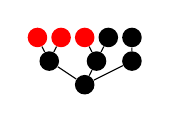
\begin{tikzpicture}[scale=.2]
\node[circle, scale=0.75, fill] (tid0) at (3.75,0){};
\node[circle, scale=0.75, fill] (tid1) at (1.5,1.5){};
\node[circle, scale=0.75, fill, red] (tid4) at (0.75,3){};
\node[circle, scale=0.75, fill, red] (tid5) at (2.25,3){};
\draw[](tid1) -- (tid4);
\draw[](tid1) -- (tid5);
\node[circle, scale=0.75, fill] (tid2) at (4.5,1.5){};
\node[circle, scale=0.75, fill, red] (tid6) at (3.75,3){};
\node[circle, scale=0.75, fill] (tid7) at (5.25,3){};
\draw[](tid2) -- (tid6);
\draw[](tid2) -- (tid7);
\node[circle, scale=0.75, fill] (tid3) at (6.75,1.5){};
\node[circle, scale=0.75, fill] (tid8) at (6.75,3){};
\draw[](tid3) -- (tid8);
\draw[](tid0) -- (tid1);
\draw[](tid0) -- (tid2);
\draw[](tid0) -- (tid3);

\end{tikzpicture}
\nodepart{two}
\footnotesize{4.87551}
\nodepart{three}
\footnotesize{0.5 0.33 0.17}
};
\node[draw=black, rectangle split, rectangle split parts=3] (sn0x9cb7238W-31) at (-31, -36) {
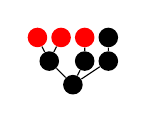
\begin{tikzpicture}[scale=.2]
\node[circle, scale=0.75, fill] (tid0) at (3,0){};
\node[circle, scale=0.75, fill] (tid1) at (1.5,1.5){};
\node[circle, scale=0.75, fill, red] (tid4) at (0.75,3){};
\node[circle, scale=0.75, fill, red] (tid5) at (2.25,3){};
\draw[](tid1) -- (tid4);
\draw[](tid1) -- (tid5);
\node[circle, scale=0.75, fill] (tid2) at (3.75,1.5){};
\node[circle, scale=0.75, fill, red] (tid6) at (3.75,3){};
\draw[](tid2) -- (tid6);
\node[circle, scale=0.75, fill] (tid3) at (5.25,1.5){};
\node[circle, scale=0.75, fill] (tid7) at (5.25,3){};
\draw[](tid3) -- (tid7);
\draw[](tid0) -- (tid1);
\draw[](tid0) -- (tid2);
\draw[](tid0) -- (tid3);

\end{tikzpicture}
\nodepart{two}
\footnotesize{4.54321}
\nodepart{three}
\footnotesize{0.67 0.33}
};
\node[draw=black, rectangle split, rectangle split parts=3] (sn0x9cb74e8W-12) at (-12, -48) {
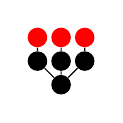
\begin{tikzpicture}[scale=.2]
\node[circle, scale=0.75, fill] (tid0) at (2.25,0){};
\node[circle, scale=0.75, fill] (tid1) at (0.75,1.5){};
\node[circle, scale=0.75, fill, red] (tid4) at (0.75,3){};
\draw[](tid1) -- (tid4);
\node[circle, scale=0.75, fill] (tid2) at (2.25,1.5){};
\node[circle, scale=0.75, fill, red] (tid5) at (2.25,3){};
\draw[](tid2) -- (tid5);
\node[circle, scale=0.75, fill] (tid3) at (3.75,1.5){};
\node[circle, scale=0.75, fill, red] (tid6) at (3.75,3){};
\draw[](tid3) -- (tid6);
\draw[](tid0) -- (tid1);
\draw[](tid0) -- (tid2);
\draw[](tid0) -- (tid3);

\end{tikzpicture}
\nodepart{two}
\footnotesize{4.21296}
\nodepart{three}
\footnotesize{1}
};
\node[draw=black, rectangle split, rectangle split parts=3] (sn0x9cb6430W-7) at (-7.25, -60) {
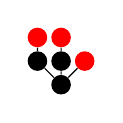
\begin{tikzpicture}[scale=.2]
\node[circle, scale=0.75, fill] (tid0) at (2.25,0){};
\node[circle, scale=0.75, fill] (tid1) at (0.75,1.5){};
\node[circle, scale=0.75, fill, red] (tid4) at (0.75,3){};
\draw[](tid1) -- (tid4);
\node[circle, scale=0.75, fill] (tid2) at (2.25,1.5){};
\node[circle, scale=0.75, fill, red] (tid5) at (2.25,3){};
\draw[](tid2) -- (tid5);
\node[circle, scale=0.75, fill, red] (tid3) at (3.75,1.5){};
\draw[](tid0) -- (tid1);
\draw[](tid0) -- (tid2);
\draw[](tid0) -- (tid3);

\end{tikzpicture}
\nodepart{two}
\footnotesize{3.87963}
\nodepart{three}
\footnotesize{0.33 0.67}
};
\node[draw=black, rectangle split, rectangle split parts=3] (sn0x9cb6658W-9) at (-9, -72) {
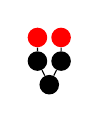
\begin{tikzpicture}[scale=.2]
\node[circle, scale=0.75, fill] (tid0) at (1.5,0){};
\node[circle, scale=0.75, fill] (tid1) at (0.75,1.5){};
\node[circle, scale=0.75, fill, red] (tid3) at (0.75,3){};
\draw[](tid1) -- (tid3);
\node[circle, scale=0.75, fill] (tid2) at (2.25,1.5){};
\node[circle, scale=0.75, fill, red] (tid4) at (2.25,3){};
\draw[](tid2) -- (tid4);
\draw[](tid0) -- (tid1);
\draw[](tid0) -- (tid2);

\end{tikzpicture}
\nodepart{two}
\footnotesize{3.75}
\nodepart{three}
\footnotesize{1}
};
\node[draw=black, rectangle split, rectangle split parts=3] (sn0x9cb6888W-8) at (-8.25, -84) {
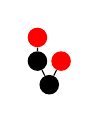
\begin{tikzpicture}[scale=.2]
\node[circle, scale=0.75, fill] (tid0) at (1.5,0){};
\node[circle, scale=0.75, fill] (tid1) at (0.75,1.5){};
\node[circle, scale=0.75, fill, red] (tid3) at (0.75,3){};
\draw[](tid1) -- (tid3);
\node[circle, scale=0.75, fill, red] (tid2) at (2.25,1.5){};
\draw[](tid0) -- (tid1);
\draw[](tid0) -- (tid2);

\end{tikzpicture}
\nodepart{two}
\footnotesize{3.25}
\nodepart{three}
\footnotesize{0.5 0.5}
};
\node[draw=black, rectangle split, rectangle split parts=3] (sn0x9cb6a00W-4) at (-4.25, -96) {
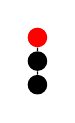
\begin{tikzpicture}[scale=.2]
\node[circle, scale=0.75, fill] (tid0) at (0.75,0){};
\node[circle, scale=0.75, fill] (tid1) at (0.75,1.5){};
\node[circle, scale=0.75, fill, red] (tid2) at (0.75,3){};
\draw[](tid1) -- (tid2);
\draw[](tid0) -- (tid1);

\end{tikzpicture}
\nodepart{two}
\footnotesize{3}
\nodepart{three}
\footnotesize{1}
};
\node[draw=black, rectangle split, rectangle split parts=3] (sn0x9cb6c28W-1) at (-1.75, -108) {

\begin{tikzpicture}[scale=.2]
\node[circle, scale=0.75, fill] (tid0) at (0.75,0){};
\node[circle, scale=0.75, fill, red] (tid1) at (0.75,1.5){};
\draw[](tid0) -- (tid1);

\end{tikzpicture}
\nodepart{two}
\footnotesize{2}
\nodepart{three}
\footnotesize{1}
};
\node[draw=black, rectangle split, rectangle split parts=3] (sn0x9cb6ca0W-1) at (-1.75, -120) {

\begin{tikzpicture}[scale=.2]
\node[circle, scale=0.75, fill, red] (tid0) at (0.75,0){};

\end{tikzpicture}
\nodepart{two}
\footnotesize{1}
\nodepart{three}
\footnotesize{}
};
\draw (sn0x9cb6c28W-1.south) -- (sn0x9cb6ca0W-1.north);
\draw (sn0x9cb6a00W-4.south) -- (sn0x9cb6c28W-1.north);
\node[draw=black, rectangle split, rectangle split parts=3] (sn0x9cb6a68W0) at (-0.75, -96) {

\begin{tikzpicture}[scale=.2]
\node[circle, scale=0.75, fill] (tid0) at (1.5,0){};
\node[circle, scale=0.75, fill, red] (tid1) at (0.75,1.5){};
\node[circle, scale=0.75, fill, red] (tid2) at (2.25,1.5){};
\draw[](tid0) -- (tid1);
\draw[](tid0) -- (tid2);

\end{tikzpicture}
\nodepart{two}
\footnotesize{2.5}
\nodepart{three}
\footnotesize{1}
};
\draw (sn0x9cb6a68W0.south) -- (sn0x9cb6c28W-1.north);
\draw (sn0x9cb6888W-8.south) -- (sn0x9cb6a00W-4.north);
\draw (sn0x9cb6888W-8.south) -- (sn0x9cb6a68W0.north);
\draw (sn0x9cb6658W-9.south) -- (sn0x9cb6888W-8.north);
\node[draw=black, rectangle split, rectangle split parts=3] (sn0x9cb66f0W-4) at (-4, -72) {
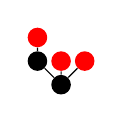
\begin{tikzpicture}[scale=.2]
\node[circle, scale=0.75, fill] (tid0) at (2.25,0){};
\node[circle, scale=0.75, fill] (tid1) at (0.75,1.5){};
\node[circle, scale=0.75, fill, red] (tid4) at (0.75,3){};
\draw[](tid1) -- (tid4);
\node[circle, scale=0.75, fill, red] (tid2) at (2.25,1.5){};
\node[circle, scale=0.75, fill, red] (tid3) at (3.75,1.5){};
\draw[](tid0) -- (tid1);
\draw[](tid0) -- (tid2);
\draw[](tid0) -- (tid3);

\end{tikzpicture}
\nodepart{two}
\footnotesize{3.44444}
\nodepart{three}
\footnotesize{0.67 0.33}
};
\node[draw=black, rectangle split, rectangle split parts=3] (sn0x9cbbc30W-3) at (-3.25, -84) {
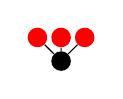
\begin{tikzpicture}[scale=.2]
\node[circle, scale=0.75, fill] (tid0) at (2.25,0){};
\node[circle, scale=0.75, fill, red] (tid1) at (0.75,1.5){};
\node[circle, scale=0.75, fill, red] (tid2) at (2.25,1.5){};
\node[circle, scale=0.75, fill, red] (tid3) at (3.75,1.5){};
\draw[](tid0) -- (tid1);
\draw[](tid0) -- (tid2);
\draw[](tid0) -- (tid3);

\end{tikzpicture}
\nodepart{two}
\footnotesize{2.83333}
\nodepart{three}
\footnotesize{1}
};
\draw (sn0x9cbbc30W-3.south) -- (sn0x9cb6a68W0.north);
\draw (sn0x9cb66f0W-4.south) -- (sn0x9cb6888W-8.north);
\draw (sn0x9cb66f0W-4.south) -- (sn0x9cbbc30W-3.north);
\draw (sn0x9cb6430W-7.south) -- (sn0x9cb6658W-9.north);
\draw (sn0x9cb6430W-7.south) -- (sn0x9cb66f0W-4.north);
\draw (sn0x9cb74e8W-12.south) -- (sn0x9cb6430W-7.north);
\node[draw=black, rectangle split, rectangle split parts=3] (sn0x9cb60d0W-5) at (-5.5, -48) {
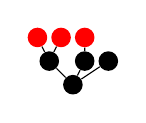
\begin{tikzpicture}[scale=.2]
\node[circle, scale=0.75, fill] (tid0) at (3,0){};
\node[circle, scale=0.75, fill] (tid1) at (1.5,1.5){};
\node[circle, scale=0.75, fill, red] (tid4) at (0.75,3){};
\node[circle, scale=0.75, fill, red] (tid5) at (2.25,3){};
\draw[](tid1) -- (tid4);
\draw[](tid1) -- (tid5);
\node[circle, scale=0.75, fill] (tid2) at (3.75,1.5){};
\node[circle, scale=0.75, fill, red] (tid6) at (3.75,3){};
\draw[](tid2) -- (tid6);
\node[circle, scale=0.75, fill] (tid3) at (5.25,1.5){};
\draw[](tid0) -- (tid1);
\draw[](tid0) -- (tid2);
\draw[](tid0) -- (tid3);

\end{tikzpicture}
\nodepart{two}
\footnotesize{4.2037}
\nodepart{three}
\footnotesize{0.67 0.33}
};
\node[draw=black, rectangle split, rectangle split parts=3] (sn0x9cbc028W0) at (-0.75, -60) {
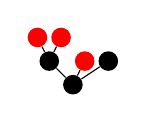
\begin{tikzpicture}[scale=.2]
\node[circle, scale=0.75, fill] (tid0) at (3,0){};
\node[circle, scale=0.75, fill] (tid1) at (1.5,1.5){};
\node[circle, scale=0.75, fill, red] (tid4) at (0.75,3){};
\node[circle, scale=0.75, fill, red] (tid5) at (2.25,3){};
\draw[](tid1) -- (tid4);
\draw[](tid1) -- (tid5);
\node[circle, scale=0.75, fill, red] (tid2) at (3.75,1.5){};
\node[circle, scale=0.75, fill] (tid3) at (5.25,1.5){};
\draw[](tid0) -- (tid1);
\draw[](tid0) -- (tid2);
\draw[](tid0) -- (tid3);

\end{tikzpicture}
\nodepart{two}
\footnotesize{3.85185}
\nodepart{three}
\footnotesize{0.33 0.67}
};
\node[draw=black, rectangle split, rectangle split parts=3] (sn0x9cbc378W2) at (2.5, -72) {
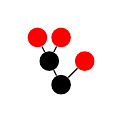
\begin{tikzpicture}[scale=.2]
\node[circle, scale=0.75, fill] (tid0) at (2.25,0){};
\node[circle, scale=0.75, fill] (tid1) at (1.5,1.5){};
\node[circle, scale=0.75, fill, red] (tid3) at (0.75,3){};
\node[circle, scale=0.75, fill, red] (tid4) at (2.25,3){};
\draw[](tid1) -- (tid3);
\draw[](tid1) -- (tid4);
\node[circle, scale=0.75, fill, red] (tid2) at (3.75,1.5){};
\draw[](tid0) -- (tid1);
\draw[](tid0) -- (tid2);

\end{tikzpicture}
\nodepart{two}
\footnotesize{3.66667}
\nodepart{three}
\footnotesize{0.33 0.67}
};
\node[draw=black, rectangle split, rectangle split parts=3] (sn0x9cbbf78W3) at (3.25, -84) {
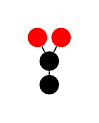
\begin{tikzpicture}[scale=.2]
\node[circle, scale=0.75, fill] (tid0) at (1.5,0){};
\node[circle, scale=0.75, fill] (tid1) at (1.5,1.5){};
\node[circle, scale=0.75, fill, red] (tid2) at (0.75,3){};
\node[circle, scale=0.75, fill, red] (tid3) at (2.25,3){};
\draw[](tid1) -- (tid2);
\draw[](tid1) -- (tid3);
\draw[](tid0) -- (tid1);

\end{tikzpicture}
\nodepart{two}
\footnotesize{3.5}
\nodepart{three}
\footnotesize{1}
};
\draw (sn0x9cbbf78W3.south) -- (sn0x9cb6a00W-4.north);
\draw (sn0x9cbc378W2.south) -- (sn0x9cbbf78W3.north);
\draw (sn0x9cbc378W2.south) -- (sn0x9cb6888W-8.north);
\draw (sn0x9cbc028W0.south) -- (sn0x9cbc378W2.north);
\draw (sn0x9cbc028W0.south) -- (sn0x9cb66f0W-4.north);
\draw (sn0x9cb60d0W-5.south) -- (sn0x9cb6430W-7.north);
\draw (sn0x9cb60d0W-5.south) -- (sn0x9cbc028W0.north);
\draw (sn0x9cb7238W-31.south) -- (sn0x9cb74e8W-12.north);
\draw (sn0x9cb7238W-31.south) -- (sn0x9cb60d0W-5.north);
\node[draw=black, rectangle split, rectangle split parts=3] (sn0x9cb6e38W-23) at (-23, -36) {
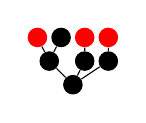
\begin{tikzpicture}[scale=.2]
\node[circle, scale=0.75, fill] (tid0) at (3,0){};
\node[circle, scale=0.75, fill] (tid1) at (1.5,1.5){};
\node[circle, scale=0.75, fill, red] (tid4) at (0.75,3){};
\node[circle, scale=0.75, fill] (tid5) at (2.25,3){};
\draw[](tid1) -- (tid4);
\draw[](tid1) -- (tid5);
\node[circle, scale=0.75, fill] (tid2) at (3.75,1.5){};
\node[circle, scale=0.75, fill, red] (tid6) at (3.75,3){};
\draw[](tid2) -- (tid6);
\node[circle, scale=0.75, fill] (tid3) at (5.25,1.5){};
\node[circle, scale=0.75, fill, red] (tid7) at (5.25,3){};
\draw[](tid3) -- (tid7);
\draw[](tid0) -- (tid1);
\draw[](tid0) -- (tid2);
\draw[](tid0) -- (tid3);

\end{tikzpicture}
\nodepart{two}
\footnotesize{4.54012}
\nodepart{three}
\footnotesize{0.33 0.67}
};
\draw (sn0x9cb6e38W-23.south) -- (sn0x9cb74e8W-12.north);
\draw (sn0x9cb6e38W-23.south) -- (sn0x9cb60d0W-5.north);
\node[draw=black, rectangle split, rectangle split parts=3] (sn0x9cbb8b0W-15) at (-15, -36) {
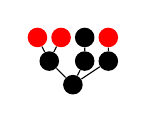
\begin{tikzpicture}[scale=.2]
\node[circle, scale=0.75, fill] (tid0) at (3,0){};
\node[circle, scale=0.75, fill] (tid1) at (1.5,1.5){};
\node[circle, scale=0.75, fill, red] (tid4) at (0.75,3){};
\node[circle, scale=0.75, fill, red] (tid5) at (2.25,3){};
\draw[](tid1) -- (tid4);
\draw[](tid1) -- (tid5);
\node[circle, scale=0.75, fill] (tid2) at (3.75,1.5){};
\node[circle, scale=0.75, fill] (tid6) at (3.75,3){};
\draw[](tid2) -- (tid6);
\node[circle, scale=0.75, fill] (tid3) at (5.25,1.5){};
\node[circle, scale=0.75, fill, red] (tid7) at (5.25,3){};
\draw[](tid3) -- (tid7);
\draw[](tid0) -- (tid1);
\draw[](tid0) -- (tid2);
\draw[](tid0) -- (tid3);

\end{tikzpicture}
\nodepart{two}
\footnotesize{4.54321}
\nodepart{three}
\footnotesize{0.67 0.33}
};
\draw (sn0x9cbb8b0W-15.south) -- (sn0x9cb74e8W-12.north);
\draw (sn0x9cbb8b0W-15.south) -- (sn0x9cb60d0W-5.north);
\draw (sn0x9cbb638W-28.south) -- (sn0x9cb7238W-31.north);
\draw (sn0x9cbb638W-28.south) -- (sn0x9cb6e38W-23.north);
\draw (sn0x9cbb638W-28.south) -- (sn0x9cbb8b0W-15.north);
\node[draw=black, rectangle split, rectangle split parts=3] (sn0x9cba0c0W-19) at (-19, -24) {
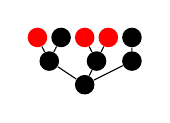
\begin{tikzpicture}[scale=.2]
\node[circle, scale=0.75, fill] (tid0) at (3.75,0){};
\node[circle, scale=0.75, fill] (tid1) at (1.5,1.5){};
\node[circle, scale=0.75, fill, red] (tid4) at (0.75,3){};
\node[circle, scale=0.75, fill] (tid5) at (2.25,3){};
\draw[](tid1) -- (tid4);
\draw[](tid1) -- (tid5);
\node[circle, scale=0.75, fill] (tid2) at (4.5,1.5){};
\node[circle, scale=0.75, fill, red] (tid6) at (3.75,3){};
\node[circle, scale=0.75, fill, red] (tid7) at (5.25,3){};
\draw[](tid2) -- (tid6);
\draw[](tid2) -- (tid7);
\node[circle, scale=0.75, fill] (tid3) at (6.75,1.5){};
\node[circle, scale=0.75, fill] (tid8) at (6.75,3){};
\draw[](tid3) -- (tid8);
\draw[](tid0) -- (tid1);
\draw[](tid0) -- (tid2);
\draw[](tid0) -- (tid3);

\end{tikzpicture}
\nodepart{two}
\footnotesize{4.87551}
\nodepart{three}
\footnotesize{0.5 0.17 0.33}
};
\draw (sn0x9cba0c0W-19.south) -- (sn0x9cb7238W-31.north);
\draw (sn0x9cba0c0W-19.south) -- (sn0x9cbb8b0W-15.north);
\draw (sn0x9cba0c0W-19.south) -- (sn0x9cb6e38W-23.north);
\node[draw=black, rectangle split, rectangle split parts=3] (sn0x9cb4458W-9) at (-9.5, -24) {
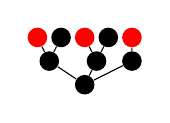
\begin{tikzpicture}[scale=.2]
\node[circle, scale=0.75, fill] (tid0) at (3.75,0){};
\node[circle, scale=0.75, fill] (tid1) at (1.5,1.5){};
\node[circle, scale=0.75, fill, red] (tid4) at (0.75,3){};
\node[circle, scale=0.75, fill] (tid5) at (2.25,3){};
\draw[](tid1) -- (tid4);
\draw[](tid1) -- (tid5);
\node[circle, scale=0.75, fill] (tid2) at (4.5,1.5){};
\node[circle, scale=0.75, fill, red] (tid6) at (3.75,3){};
\node[circle, scale=0.75, fill] (tid7) at (5.25,3){};
\draw[](tid2) -- (tid6);
\draw[](tid2) -- (tid7);
\node[circle, scale=0.75, fill] (tid3) at (6.75,1.5){};
\node[circle, scale=0.75, fill, red] (tid8) at (6.75,3){};
\draw[](tid3) -- (tid8);
\draw[](tid0) -- (tid1);
\draw[](tid0) -- (tid2);
\draw[](tid0) -- (tid3);

\end{tikzpicture}
\nodepart{two}
\footnotesize{4.87346}
\nodepart{three}
\footnotesize{0.33 0.33 0.17 0.17}
};
\node[draw=black, rectangle split, rectangle split parts=3] (sn0x9cbc8f8W-7) at (-7, -36) {
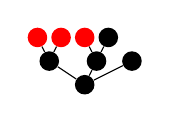
\begin{tikzpicture}[scale=.2]
\node[circle, scale=0.75, fill] (tid0) at (3.75,0){};
\node[circle, scale=0.75, fill] (tid1) at (1.5,1.5){};
\node[circle, scale=0.75, fill, red] (tid4) at (0.75,3){};
\node[circle, scale=0.75, fill, red] (tid5) at (2.25,3){};
\draw[](tid1) -- (tid4);
\draw[](tid1) -- (tid5);
\node[circle, scale=0.75, fill] (tid2) at (4.5,1.5){};
\node[circle, scale=0.75, fill, red] (tid6) at (3.75,3){};
\node[circle, scale=0.75, fill] (tid7) at (5.25,3){};
\draw[](tid2) -- (tid6);
\draw[](tid2) -- (tid7);
\node[circle, scale=0.75, fill] (tid3) at (6.75,1.5){};
\draw[](tid0) -- (tid1);
\draw[](tid0) -- (tid2);
\draw[](tid0) -- (tid3);

\end{tikzpicture}
\nodepart{two}
\footnotesize{4.53704}
\nodepart{three}
\footnotesize{1}
};
\draw (sn0x9cbc8f8W-7.south) -- (sn0x9cb60d0W-5.north);
\node[draw=black, rectangle split, rectangle split parts=3] (sn0x9cbcbe0W2) at (2.5, -36) {
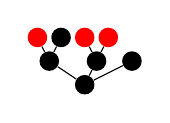
\begin{tikzpicture}[scale=.2]
\node[circle, scale=0.75, fill] (tid0) at (3.75,0){};
\node[circle, scale=0.75, fill] (tid1) at (1.5,1.5){};
\node[circle, scale=0.75, fill, red] (tid4) at (0.75,3){};
\node[circle, scale=0.75, fill] (tid5) at (2.25,3){};
\draw[](tid1) -- (tid4);
\draw[](tid1) -- (tid5);
\node[circle, scale=0.75, fill] (tid2) at (4.5,1.5){};
\node[circle, scale=0.75, fill, red] (tid6) at (3.75,3){};
\node[circle, scale=0.75, fill, red] (tid7) at (5.25,3){};
\draw[](tid2) -- (tid6);
\draw[](tid2) -- (tid7);
\node[circle, scale=0.75, fill] (tid3) at (6.75,1.5){};
\draw[](tid0) -- (tid1);
\draw[](tid0) -- (tid2);
\draw[](tid0) -- (tid3);

\end{tikzpicture}
\nodepart{two}
\footnotesize{4.53704}
\nodepart{three}
\footnotesize{1}
};
\draw (sn0x9cbcbe0W2.south) -- (sn0x9cb60d0W-5.north);
\draw (sn0x9cb4458W-9.south) -- (sn0x9cb6e38W-23.north);
\draw (sn0x9cb4458W-9.south) -- (sn0x9cbb8b0W-15.north);
\draw (sn0x9cb4458W-9.south) -- (sn0x9cbc8f8W-7.north);
\draw (sn0x9cb4458W-9.south) -- (sn0x9cbcbe0W2.north);
\node[draw=black, rectangle split, rectangle split parts=3] (sn0x9cb4170W0) at (0, -24) {
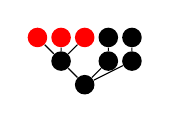
\begin{tikzpicture}[scale=.2]
\node[circle, scale=0.75, fill] (tid0) at (3.75,0){};
\node[circle, scale=0.75, fill] (tid1) at (2.25,1.5){};
\node[circle, scale=0.75, fill, red] (tid4) at (0.75,3){};
\node[circle, scale=0.75, fill, red] (tid5) at (2.25,3){};
\node[circle, scale=0.75, fill, red] (tid6) at (3.75,3){};
\draw[](tid1) -- (tid4);
\draw[](tid1) -- (tid5);
\draw[](tid1) -- (tid6);
\node[circle, scale=0.75, fill] (tid2) at (5.25,1.5){};
\node[circle, scale=0.75, fill] (tid7) at (5.25,3){};
\draw[](tid2) -- (tid7);
\node[circle, scale=0.75, fill] (tid3) at (6.75,1.5){};
\node[circle, scale=0.75, fill] (tid8) at (6.75,3){};
\draw[](tid3) -- (tid8);
\draw[](tid0) -- (tid1);
\draw[](tid0) -- (tid2);
\draw[](tid0) -- (tid3);

\end{tikzpicture}
\nodepart{two}
\footnotesize{4.87654}
\nodepart{three}
\footnotesize{0.5 0.5}
};
\draw (sn0x9cb4170W0.south) -- (sn0x9cb7238W-31.north);
\draw (sn0x9cb4170W0.south) -- (sn0x9cbb8b0W-15.north);
\node[draw=black, rectangle split, rectangle split parts=3] (sn0x9cb4fa8W9) at (9.5, -24) {
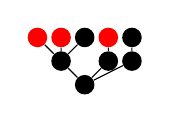
\begin{tikzpicture}[scale=.2]
\node[circle, scale=0.75, fill] (tid0) at (3.75,0){};
\node[circle, scale=0.75, fill] (tid1) at (2.25,1.5){};
\node[circle, scale=0.75, fill, red] (tid4) at (0.75,3){};
\node[circle, scale=0.75, fill, red] (tid5) at (2.25,3){};
\node[circle, scale=0.75, fill] (tid6) at (3.75,3){};
\draw[](tid1) -- (tid4);
\draw[](tid1) -- (tid5);
\draw[](tid1) -- (tid6);
\node[circle, scale=0.75, fill] (tid2) at (5.25,1.5){};
\node[circle, scale=0.75, fill, red] (tid7) at (5.25,3){};
\draw[](tid2) -- (tid7);
\node[circle, scale=0.75, fill] (tid3) at (6.75,1.5){};
\node[circle, scale=0.75, fill] (tid8) at (6.75,3){};
\draw[](tid3) -- (tid8);
\draw[](tid0) -- (tid1);
\draw[](tid0) -- (tid2);
\draw[](tid0) -- (tid3);

\end{tikzpicture}
\nodepart{two}
\footnotesize{4.87243}
\nodepart{three}
\footnotesize{0.33 0.33 0.17 0.17}
};
\node[draw=black, rectangle split, rectangle split parts=3] (sn0x9cbcee0W12) at (12, -36) {
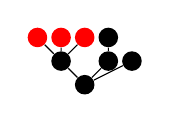
\begin{tikzpicture}[scale=.2]
\node[circle, scale=0.75, fill] (tid0) at (3.75,0){};
\node[circle, scale=0.75, fill] (tid1) at (2.25,1.5){};
\node[circle, scale=0.75, fill, red] (tid4) at (0.75,3){};
\node[circle, scale=0.75, fill, red] (tid5) at (2.25,3){};
\node[circle, scale=0.75, fill, red] (tid6) at (3.75,3){};
\draw[](tid1) -- (tid4);
\draw[](tid1) -- (tid5);
\draw[](tid1) -- (tid6);
\node[circle, scale=0.75, fill] (tid2) at (5.25,1.5){};
\node[circle, scale=0.75, fill] (tid7) at (5.25,3){};
\draw[](tid2) -- (tid7);
\node[circle, scale=0.75, fill] (tid3) at (6.75,1.5){};
\draw[](tid0) -- (tid1);
\draw[](tid0) -- (tid2);
\draw[](tid0) -- (tid3);

\end{tikzpicture}
\nodepart{two}
\footnotesize{4.53704}
\nodepart{three}
\footnotesize{1}
};
\draw (sn0x9cbcee0W12.south) -- (sn0x9cb60d0W-5.north);
\node[draw=black, rectangle split, rectangle split parts=3] (sn0x9cbd338W21) at (21.5, -36) {
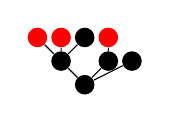
\begin{tikzpicture}[scale=.2]
\node[circle, scale=0.75, fill] (tid0) at (3.75,0){};
\node[circle, scale=0.75, fill] (tid1) at (2.25,1.5){};
\node[circle, scale=0.75, fill, red] (tid4) at (0.75,3){};
\node[circle, scale=0.75, fill, red] (tid5) at (2.25,3){};
\node[circle, scale=0.75, fill] (tid6) at (3.75,3){};
\draw[](tid1) -- (tid4);
\draw[](tid1) -- (tid5);
\draw[](tid1) -- (tid6);
\node[circle, scale=0.75, fill] (tid2) at (5.25,1.5){};
\node[circle, scale=0.75, fill, red] (tid7) at (5.25,3){};
\draw[](tid2) -- (tid7);
\node[circle, scale=0.75, fill] (tid3) at (6.75,1.5){};
\draw[](tid0) -- (tid1);
\draw[](tid0) -- (tid2);
\draw[](tid0) -- (tid3);

\end{tikzpicture}
\nodepart{two}
\footnotesize{4.53086}
\nodepart{three}
\footnotesize{0.67 0.33}
};
\node[draw=black, rectangle split, rectangle split parts=3] (sn0x9cbd5b0W2) at (2.5, -48) {
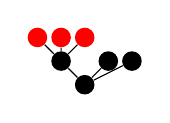
\begin{tikzpicture}[scale=.2]
\node[circle, scale=0.75, fill] (tid0) at (3.75,0){};
\node[circle, scale=0.75, fill] (tid1) at (2.25,1.5){};
\node[circle, scale=0.75, fill, red] (tid4) at (0.75,3){};
\node[circle, scale=0.75, fill, red] (tid5) at (2.25,3){};
\node[circle, scale=0.75, fill, red] (tid6) at (3.75,3){};
\draw[](tid1) -- (tid4);
\draw[](tid1) -- (tid5);
\draw[](tid1) -- (tid6);
\node[circle, scale=0.75, fill] (tid2) at (5.25,1.5){};
\node[circle, scale=0.75, fill] (tid3) at (6.75,1.5){};
\draw[](tid0) -- (tid1);
\draw[](tid0) -- (tid2);
\draw[](tid0) -- (tid3);

\end{tikzpicture}
\nodepart{two}
\footnotesize{4.18519}
\nodepart{three}
\footnotesize{1}
};
\draw (sn0x9cbd5b0W2.south) -- (sn0x9cbc028W0.north);
\draw (sn0x9cbd338W21.south) -- (sn0x9cb60d0W-5.north);
\draw (sn0x9cbd338W21.south) -- (sn0x9cbd5b0W2.north);
\draw (sn0x9cb4fa8W9.south) -- (sn0x9cb7238W-31.north);
\draw (sn0x9cb4fa8W9.south) -- (sn0x9cb6e38W-23.north);
\draw (sn0x9cb4fa8W9.south) -- (sn0x9cbcee0W12.north);
\draw (sn0x9cb4fa8W9.south) -- (sn0x9cbd338W21.north);
\node[draw=black, rectangle split, rectangle split parts=3] (sn0x9cbba18W19) at (19, -24) {
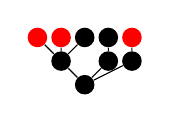
\begin{tikzpicture}[scale=.2]
\node[circle, scale=0.75, fill] (tid0) at (3.75,0){};
\node[circle, scale=0.75, fill] (tid1) at (2.25,1.5){};
\node[circle, scale=0.75, fill, red] (tid4) at (0.75,3){};
\node[circle, scale=0.75, fill, red] (tid5) at (2.25,3){};
\node[circle, scale=0.75, fill] (tid6) at (3.75,3){};
\draw[](tid1) -- (tid4);
\draw[](tid1) -- (tid5);
\draw[](tid1) -- (tid6);
\node[circle, scale=0.75, fill] (tid2) at (5.25,1.5){};
\node[circle, scale=0.75, fill] (tid7) at (5.25,3){};
\draw[](tid2) -- (tid7);
\node[circle, scale=0.75, fill] (tid3) at (6.75,1.5){};
\node[circle, scale=0.75, fill, red] (tid8) at (6.75,3){};
\draw[](tid3) -- (tid8);
\draw[](tid0) -- (tid1);
\draw[](tid0) -- (tid2);
\draw[](tid0) -- (tid3);

\end{tikzpicture}
\nodepart{two}
\footnotesize{4.87243}
\nodepart{three}
\footnotesize{0.33 0.33 0.17 0.17}
};
\draw (sn0x9cbba18W19.south) -- (sn0x9cbb8b0W-15.north);
\draw (sn0x9cbba18W19.south) -- (sn0x9cb6e38W-23.north);
\draw (sn0x9cbba18W19.south) -- (sn0x9cbcee0W12.north);
\draw (sn0x9cbba18W19.south) -- (sn0x9cbd338W21.north);
\draw (sn0x9cb56b0W-5.south) -- (sn0x9cbb638W-28.north);
\draw (sn0x9cb56b0W-5.south) -- (sn0x9cba0c0W-19.north);
\draw (sn0x9cb56b0W-5.south) -- (sn0x9cb4458W-9.north);
\draw (sn0x9cb56b0W-5.south) -- (sn0x9cb4170W0.north);
\draw (sn0x9cb56b0W-5.south) -- (sn0x9cb4fa8W9.north);
\draw (sn0x9cb56b0W-5.south) -- (sn0x9cbba18W19.north);
\end{tikzpicture}

%%% Local Variables:
%%% TeX-master: "thesis/thesis.tex"
%%% End: 

\begin{tikzpicture}[scale=.2, anchor=south west]
\node[draw=black, rectangle split, rectangle split parts=3] (sn0x9cb5710W-5) at (-5.5, -12) {
\begin{tikzpicture}[scale=.2]
\node[circle, scale=0.75, fill] (tid0) at (4.5,0){};
\node[circle, scale=0.75, fill] (tid1) at (2.25,1.5){};
\node[circle, scale=0.75, fill, red] (tid4) at (0.75,3){};
\node[circle, scale=0.75, fill, red] (tid5) at (2.25,3){};
\node[circle, scale=0.75, fill] (tid6) at (3.75,3){};
\draw[](tid1) -- (tid4);
\draw[](tid1) -- (tid5);
\draw[](tid1) -- (tid6);
\node[circle, scale=0.75, fill] (tid2) at (6,1.5){};
\node[circle, scale=0.75, fill] (tid7) at (5.25,3){};
\node[circle, scale=0.75, fill] (tid8) at (6.75,3){};
\draw[](tid2) -- (tid7);
\draw[](tid2) -- (tid8);
\node[circle, scale=0.75, fill] (tid3) at (8.25,1.5){};
\node[circle, scale=0.75, fill, red] (tid9) at (8.25,3){};
\draw[](tid3) -- (tid9);
\draw[](tid0) -- (tid1);
\draw[](tid0) -- (tid2);
\draw[](tid0) -- (tid3);

\end{tikzpicture}
\nodepart{two}
\footnotesize{5.20531}
\nodepart{three}
\footnotesize{0.22 0.44 0.11 0.22}
};
\node[draw=black, rectangle split, rectangle split parts=3] (sn0x9cbdb40W-20) at (-20.5, -24) {
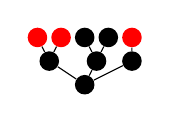
\begin{tikzpicture}[scale=.2]
\node[circle, scale=0.75, fill] (tid0) at (3.75,0){};
\node[circle, scale=0.75, fill] (tid1) at (1.5,1.5){};
\node[circle, scale=0.75, fill, red] (tid4) at (0.75,3){};
\node[circle, scale=0.75, fill, red] (tid5) at (2.25,3){};
\draw[](tid1) -- (tid4);
\draw[](tid1) -- (tid5);
\node[circle, scale=0.75, fill] (tid2) at (4.5,1.5){};
\node[circle, scale=0.75, fill] (tid6) at (3.75,3){};
\node[circle, scale=0.75, fill] (tid7) at (5.25,3){};
\draw[](tid2) -- (tid6);
\draw[](tid2) -- (tid7);
\node[circle, scale=0.75, fill] (tid3) at (6.75,1.5){};
\node[circle, scale=0.75, fill, red] (tid8) at (6.75,3){};
\draw[](tid3) -- (tid8);
\draw[](tid0) -- (tid1);
\draw[](tid0) -- (tid2);
\draw[](tid0) -- (tid3);

\end{tikzpicture}
\nodepart{two}
\footnotesize{4.87243}
\nodepart{three}
\footnotesize{0.67 0.33}
};
\node[draw=black, rectangle split, rectangle split parts=3] (sn0x9cb6e38W-27) at (-27, -36) {
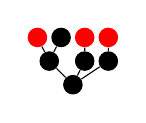
\begin{tikzpicture}[scale=.2]
\node[circle, scale=0.75, fill] (tid0) at (3,0){};
\node[circle, scale=0.75, fill] (tid1) at (1.5,1.5){};
\node[circle, scale=0.75, fill, red] (tid4) at (0.75,3){};
\node[circle, scale=0.75, fill] (tid5) at (2.25,3){};
\draw[](tid1) -- (tid4);
\draw[](tid1) -- (tid5);
\node[circle, scale=0.75, fill] (tid2) at (3.75,1.5){};
\node[circle, scale=0.75, fill, red] (tid6) at (3.75,3){};
\draw[](tid2) -- (tid6);
\node[circle, scale=0.75, fill] (tid3) at (5.25,1.5){};
\node[circle, scale=0.75, fill, red] (tid7) at (5.25,3){};
\draw[](tid3) -- (tid7);
\draw[](tid0) -- (tid1);
\draw[](tid0) -- (tid2);
\draw[](tid0) -- (tid3);

\end{tikzpicture}
\nodepart{two}
\footnotesize{4.54012}
\nodepart{three}
\footnotesize{0.33 0.67}
};
\node[draw=black, rectangle split, rectangle split parts=3] (sn0x9cb74e8W-12) at (-12, -48) {
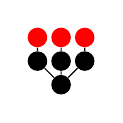
\begin{tikzpicture}[scale=.2]
\node[circle, scale=0.75, fill] (tid0) at (2.25,0){};
\node[circle, scale=0.75, fill] (tid1) at (0.75,1.5){};
\node[circle, scale=0.75, fill, red] (tid4) at (0.75,3){};
\draw[](tid1) -- (tid4);
\node[circle, scale=0.75, fill] (tid2) at (2.25,1.5){};
\node[circle, scale=0.75, fill, red] (tid5) at (2.25,3){};
\draw[](tid2) -- (tid5);
\node[circle, scale=0.75, fill] (tid3) at (3.75,1.5){};
\node[circle, scale=0.75, fill, red] (tid6) at (3.75,3){};
\draw[](tid3) -- (tid6);
\draw[](tid0) -- (tid1);
\draw[](tid0) -- (tid2);
\draw[](tid0) -- (tid3);

\end{tikzpicture}
\nodepart{two}
\footnotesize{4.21296}
\nodepart{three}
\footnotesize{1}
};
\node[draw=black, rectangle split, rectangle split parts=3] (sn0x9cb6430W-7) at (-7.25, -60) {
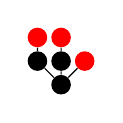
\begin{tikzpicture}[scale=.2]
\node[circle, scale=0.75, fill] (tid0) at (2.25,0){};
\node[circle, scale=0.75, fill] (tid1) at (0.75,1.5){};
\node[circle, scale=0.75, fill, red] (tid4) at (0.75,3){};
\draw[](tid1) -- (tid4);
\node[circle, scale=0.75, fill] (tid2) at (2.25,1.5){};
\node[circle, scale=0.75, fill, red] (tid5) at (2.25,3){};
\draw[](tid2) -- (tid5);
\node[circle, scale=0.75, fill, red] (tid3) at (3.75,1.5){};
\draw[](tid0) -- (tid1);
\draw[](tid0) -- (tid2);
\draw[](tid0) -- (tid3);

\end{tikzpicture}
\nodepart{two}
\footnotesize{3.87963}
\nodepart{three}
\footnotesize{0.33 0.67}
};
\node[draw=black, rectangle split, rectangle split parts=3] (sn0x9cb6658W-9) at (-9, -72) {
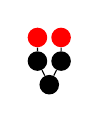
\begin{tikzpicture}[scale=.2]
\node[circle, scale=0.75, fill] (tid0) at (1.5,0){};
\node[circle, scale=0.75, fill] (tid1) at (0.75,1.5){};
\node[circle, scale=0.75, fill, red] (tid3) at (0.75,3){};
\draw[](tid1) -- (tid3);
\node[circle, scale=0.75, fill] (tid2) at (2.25,1.5){};
\node[circle, scale=0.75, fill, red] (tid4) at (2.25,3){};
\draw[](tid2) -- (tid4);
\draw[](tid0) -- (tid1);
\draw[](tid0) -- (tid2);

\end{tikzpicture}
\nodepart{two}
\footnotesize{3.75}
\nodepart{three}
\footnotesize{1}
};
\node[draw=black, rectangle split, rectangle split parts=3] (sn0x9cb6888W-8) at (-8.25, -84) {
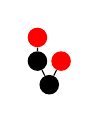
\begin{tikzpicture}[scale=.2]
\node[circle, scale=0.75, fill] (tid0) at (1.5,0){};
\node[circle, scale=0.75, fill] (tid1) at (0.75,1.5){};
\node[circle, scale=0.75, fill, red] (tid3) at (0.75,3){};
\draw[](tid1) -- (tid3);
\node[circle, scale=0.75, fill, red] (tid2) at (2.25,1.5){};
\draw[](tid0) -- (tid1);
\draw[](tid0) -- (tid2);

\end{tikzpicture}
\nodepart{two}
\footnotesize{3.25}
\nodepart{three}
\footnotesize{0.5 0.5}
};
\node[draw=black, rectangle split, rectangle split parts=3] (sn0x9cb6a00W-4) at (-4.25, -96) {
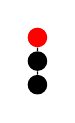
\begin{tikzpicture}[scale=.2]
\node[circle, scale=0.75, fill] (tid0) at (0.75,0){};
\node[circle, scale=0.75, fill] (tid1) at (0.75,1.5){};
\node[circle, scale=0.75, fill, red] (tid2) at (0.75,3){};
\draw[](tid1) -- (tid2);
\draw[](tid0) -- (tid1);

\end{tikzpicture}
\nodepart{two}
\footnotesize{3}
\nodepart{three}
\footnotesize{1}
};
\node[draw=black, rectangle split, rectangle split parts=3] (sn0x9cb6c28W-1) at (-1.75, -108) {

\begin{tikzpicture}[scale=.2]
\node[circle, scale=0.75, fill] (tid0) at (0.75,0){};
\node[circle, scale=0.75, fill, red] (tid1) at (0.75,1.5){};
\draw[](tid0) -- (tid1);

\end{tikzpicture}
\nodepart{two}
\footnotesize{2}
\nodepart{three}
\footnotesize{1}
};
\node[draw=black, rectangle split, rectangle split parts=3] (sn0x9cb6ca0W-1) at (-1.75, -120) {

\begin{tikzpicture}[scale=.2]
\node[circle, scale=0.75, fill, red] (tid0) at (0.75,0){};

\end{tikzpicture}
\nodepart{two}
\footnotesize{1}
\nodepart{three}
\footnotesize{}
};
\draw (sn0x9cb6c28W-1.south) -- (sn0x9cb6ca0W-1.north);
\draw (sn0x9cb6a00W-4.south) -- (sn0x9cb6c28W-1.north);
\node[draw=black, rectangle split, rectangle split parts=3] (sn0x9cb6a68W0) at (-0.75, -96) {

\begin{tikzpicture}[scale=.2]
\node[circle, scale=0.75, fill] (tid0) at (1.5,0){};
\node[circle, scale=0.75, fill, red] (tid1) at (0.75,1.5){};
\node[circle, scale=0.75, fill, red] (tid2) at (2.25,1.5){};
\draw[](tid0) -- (tid1);
\draw[](tid0) -- (tid2);

\end{tikzpicture}
\nodepart{two}
\footnotesize{2.5}
\nodepart{three}
\footnotesize{1}
};
\draw (sn0x9cb6a68W0.south) -- (sn0x9cb6c28W-1.north);
\draw (sn0x9cb6888W-8.south) -- (sn0x9cb6a00W-4.north);
\draw (sn0x9cb6888W-8.south) -- (sn0x9cb6a68W0.north);
\draw (sn0x9cb6658W-9.south) -- (sn0x9cb6888W-8.north);
\node[draw=black, rectangle split, rectangle split parts=3] (sn0x9cb66f0W-4) at (-4, -72) {
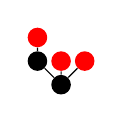
\begin{tikzpicture}[scale=.2]
\node[circle, scale=0.75, fill] (tid0) at (2.25,0){};
\node[circle, scale=0.75, fill] (tid1) at (0.75,1.5){};
\node[circle, scale=0.75, fill, red] (tid4) at (0.75,3){};
\draw[](tid1) -- (tid4);
\node[circle, scale=0.75, fill, red] (tid2) at (2.25,1.5){};
\node[circle, scale=0.75, fill, red] (tid3) at (3.75,1.5){};
\draw[](tid0) -- (tid1);
\draw[](tid0) -- (tid2);
\draw[](tid0) -- (tid3);

\end{tikzpicture}
\nodepart{two}
\footnotesize{3.44444}
\nodepart{three}
\footnotesize{0.67 0.33}
};
\node[draw=black, rectangle split, rectangle split parts=3] (sn0x9cbbc30W-3) at (-3.25, -84) {
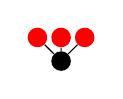
\begin{tikzpicture}[scale=.2]
\node[circle, scale=0.75, fill] (tid0) at (2.25,0){};
\node[circle, scale=0.75, fill, red] (tid1) at (0.75,1.5){};
\node[circle, scale=0.75, fill, red] (tid2) at (2.25,1.5){};
\node[circle, scale=0.75, fill, red] (tid3) at (3.75,1.5){};
\draw[](tid0) -- (tid1);
\draw[](tid0) -- (tid2);
\draw[](tid0) -- (tid3);

\end{tikzpicture}
\nodepart{two}
\footnotesize{2.83333}
\nodepart{three}
\footnotesize{1}
};
\draw (sn0x9cbbc30W-3.south) -- (sn0x9cb6a68W0.north);
\draw (sn0x9cb66f0W-4.south) -- (sn0x9cb6888W-8.north);
\draw (sn0x9cb66f0W-4.south) -- (sn0x9cbbc30W-3.north);
\draw (sn0x9cb6430W-7.south) -- (sn0x9cb6658W-9.north);
\draw (sn0x9cb6430W-7.south) -- (sn0x9cb66f0W-4.north);
\draw (sn0x9cb74e8W-12.south) -- (sn0x9cb6430W-7.north);
\node[draw=black, rectangle split, rectangle split parts=3] (sn0x9cb60d0W-5) at (-5.5, -48) {
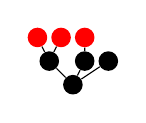
\begin{tikzpicture}[scale=.2]
\node[circle, scale=0.75, fill] (tid0) at (3,0){};
\node[circle, scale=0.75, fill] (tid1) at (1.5,1.5){};
\node[circle, scale=0.75, fill, red] (tid4) at (0.75,3){};
\node[circle, scale=0.75, fill, red] (tid5) at (2.25,3){};
\draw[](tid1) -- (tid4);
\draw[](tid1) -- (tid5);
\node[circle, scale=0.75, fill] (tid2) at (3.75,1.5){};
\node[circle, scale=0.75, fill, red] (tid6) at (3.75,3){};
\draw[](tid2) -- (tid6);
\node[circle, scale=0.75, fill] (tid3) at (5.25,1.5){};
\draw[](tid0) -- (tid1);
\draw[](tid0) -- (tid2);
\draw[](tid0) -- (tid3);

\end{tikzpicture}
\nodepart{two}
\footnotesize{4.2037}
\nodepart{three}
\footnotesize{0.67 0.33}
};
\node[draw=black, rectangle split, rectangle split parts=3] (sn0x9cbc028W0) at (-0.75, -60) {
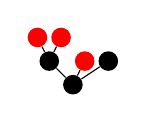
\begin{tikzpicture}[scale=.2]
\node[circle, scale=0.75, fill] (tid0) at (3,0){};
\node[circle, scale=0.75, fill] (tid1) at (1.5,1.5){};
\node[circle, scale=0.75, fill, red] (tid4) at (0.75,3){};
\node[circle, scale=0.75, fill, red] (tid5) at (2.25,3){};
\draw[](tid1) -- (tid4);
\draw[](tid1) -- (tid5);
\node[circle, scale=0.75, fill, red] (tid2) at (3.75,1.5){};
\node[circle, scale=0.75, fill] (tid3) at (5.25,1.5){};
\draw[](tid0) -- (tid1);
\draw[](tid0) -- (tid2);
\draw[](tid0) -- (tid3);

\end{tikzpicture}
\nodepart{two}
\footnotesize{3.85185}
\nodepart{three}
\footnotesize{0.33 0.67}
};
\node[draw=black, rectangle split, rectangle split parts=3] (sn0x9cbc378W2) at (2.5, -72) {
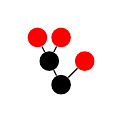
\begin{tikzpicture}[scale=.2]
\node[circle, scale=0.75, fill] (tid0) at (2.25,0){};
\node[circle, scale=0.75, fill] (tid1) at (1.5,1.5){};
\node[circle, scale=0.75, fill, red] (tid3) at (0.75,3){};
\node[circle, scale=0.75, fill, red] (tid4) at (2.25,3){};
\draw[](tid1) -- (tid3);
\draw[](tid1) -- (tid4);
\node[circle, scale=0.75, fill, red] (tid2) at (3.75,1.5){};
\draw[](tid0) -- (tid1);
\draw[](tid0) -- (tid2);

\end{tikzpicture}
\nodepart{two}
\footnotesize{3.66667}
\nodepart{three}
\footnotesize{0.33 0.67}
};
\node[draw=black, rectangle split, rectangle split parts=3] (sn0x9cbbf78W3) at (3.25, -84) {
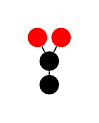
\begin{tikzpicture}[scale=.2]
\node[circle, scale=0.75, fill] (tid0) at (1.5,0){};
\node[circle, scale=0.75, fill] (tid1) at (1.5,1.5){};
\node[circle, scale=0.75, fill, red] (tid2) at (0.75,3){};
\node[circle, scale=0.75, fill, red] (tid3) at (2.25,3){};
\draw[](tid1) -- (tid2);
\draw[](tid1) -- (tid3);
\draw[](tid0) -- (tid1);

\end{tikzpicture}
\nodepart{two}
\footnotesize{3.5}
\nodepart{three}
\footnotesize{1}
};
\draw (sn0x9cbbf78W3.south) -- (sn0x9cb6a00W-4.north);
\draw (sn0x9cbc378W2.south) -- (sn0x9cbbf78W3.north);
\draw (sn0x9cbc378W2.south) -- (sn0x9cb6888W-8.north);
\draw (sn0x9cbc028W0.south) -- (sn0x9cbc378W2.north);
\draw (sn0x9cbc028W0.south) -- (sn0x9cb66f0W-4.north);
\draw (sn0x9cb60d0W-5.south) -- (sn0x9cb6430W-7.north);
\draw (sn0x9cb60d0W-5.south) -- (sn0x9cbc028W0.north);
\draw (sn0x9cb6e38W-27.south) -- (sn0x9cb74e8W-12.north);
\draw (sn0x9cb6e38W-27.south) -- (sn0x9cb60d0W-5.north);
\node[draw=black, rectangle split, rectangle split parts=3] (sn0x9cbc8f8W-19) at (-19, -36) {
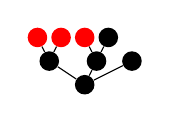
\begin{tikzpicture}[scale=.2]
\node[circle, scale=0.75, fill] (tid0) at (3.75,0){};
\node[circle, scale=0.75, fill] (tid1) at (1.5,1.5){};
\node[circle, scale=0.75, fill, red] (tid4) at (0.75,3){};
\node[circle, scale=0.75, fill, red] (tid5) at (2.25,3){};
\draw[](tid1) -- (tid4);
\draw[](tid1) -- (tid5);
\node[circle, scale=0.75, fill] (tid2) at (4.5,1.5){};
\node[circle, scale=0.75, fill, red] (tid6) at (3.75,3){};
\node[circle, scale=0.75, fill] (tid7) at (5.25,3){};
\draw[](tid2) -- (tid6);
\draw[](tid2) -- (tid7);
\node[circle, scale=0.75, fill] (tid3) at (6.75,1.5){};
\draw[](tid0) -- (tid1);
\draw[](tid0) -- (tid2);
\draw[](tid0) -- (tid3);

\end{tikzpicture}
\nodepart{two}
\footnotesize{4.53704}
\nodepart{three}
\footnotesize{1}
};
\draw (sn0x9cbc8f8W-19.south) -- (sn0x9cb60d0W-5.north);
\draw (sn0x9cbdb40W-20.south) -- (sn0x9cb6e38W-27.north);
\draw (sn0x9cbdb40W-20.south) -- (sn0x9cbc8f8W-19.north);
\node[draw=black, rectangle split, rectangle split parts=3] (sn0x9cb4458W-11) at (-11, -24) {
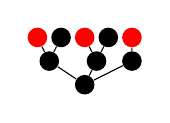
\begin{tikzpicture}[scale=.2]
\node[circle, scale=0.75, fill] (tid0) at (3.75,0){};
\node[circle, scale=0.75, fill] (tid1) at (1.5,1.5){};
\node[circle, scale=0.75, fill, red] (tid4) at (0.75,3){};
\node[circle, scale=0.75, fill] (tid5) at (2.25,3){};
\draw[](tid1) -- (tid4);
\draw[](tid1) -- (tid5);
\node[circle, scale=0.75, fill] (tid2) at (4.5,1.5){};
\node[circle, scale=0.75, fill, red] (tid6) at (3.75,3){};
\node[circle, scale=0.75, fill] (tid7) at (5.25,3){};
\draw[](tid2) -- (tid6);
\draw[](tid2) -- (tid7);
\node[circle, scale=0.75, fill] (tid3) at (6.75,1.5){};
\node[circle, scale=0.75, fill, red] (tid8) at (6.75,3){};
\draw[](tid3) -- (tid8);
\draw[](tid0) -- (tid1);
\draw[](tid0) -- (tid2);
\draw[](tid0) -- (tid3);

\end{tikzpicture}
\nodepart{two}
\footnotesize{4.87346}
\nodepart{three}
\footnotesize{0.33 0.33 0.17 0.17}
};
\node[draw=black, rectangle split, rectangle split parts=3] (sn0x9cbb8b0W-9) at (-9.5, -36) {
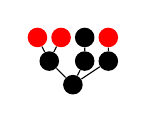
\begin{tikzpicture}[scale=.2]
\node[circle, scale=0.75, fill] (tid0) at (3,0){};
\node[circle, scale=0.75, fill] (tid1) at (1.5,1.5){};
\node[circle, scale=0.75, fill, red] (tid4) at (0.75,3){};
\node[circle, scale=0.75, fill, red] (tid5) at (2.25,3){};
\draw[](tid1) -- (tid4);
\draw[](tid1) -- (tid5);
\node[circle, scale=0.75, fill] (tid2) at (3.75,1.5){};
\node[circle, scale=0.75, fill] (tid6) at (3.75,3){};
\draw[](tid2) -- (tid6);
\node[circle, scale=0.75, fill] (tid3) at (5.25,1.5){};
\node[circle, scale=0.75, fill, red] (tid7) at (5.25,3){};
\draw[](tid3) -- (tid7);
\draw[](tid0) -- (tid1);
\draw[](tid0) -- (tid2);
\draw[](tid0) -- (tid3);

\end{tikzpicture}
\nodepart{two}
\footnotesize{4.54321}
\nodepart{three}
\footnotesize{0.67 0.33}
};
\draw (sn0x9cbb8b0W-9.south) -- (sn0x9cb74e8W-12.north);
\draw (sn0x9cbb8b0W-9.south) -- (sn0x9cb60d0W-5.north);
\node[draw=black, rectangle split, rectangle split parts=3] (sn0x9cbcbe0W-1) at (-1.5, -36) {
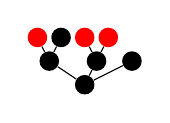
\begin{tikzpicture}[scale=.2]
\node[circle, scale=0.75, fill] (tid0) at (3.75,0){};
\node[circle, scale=0.75, fill] (tid1) at (1.5,1.5){};
\node[circle, scale=0.75, fill, red] (tid4) at (0.75,3){};
\node[circle, scale=0.75, fill] (tid5) at (2.25,3){};
\draw[](tid1) -- (tid4);
\draw[](tid1) -- (tid5);
\node[circle, scale=0.75, fill] (tid2) at (4.5,1.5){};
\node[circle, scale=0.75, fill, red] (tid6) at (3.75,3){};
\node[circle, scale=0.75, fill, red] (tid7) at (5.25,3){};
\draw[](tid2) -- (tid6);
\draw[](tid2) -- (tid7);
\node[circle, scale=0.75, fill] (tid3) at (6.75,1.5){};
\draw[](tid0) -- (tid1);
\draw[](tid0) -- (tid2);
\draw[](tid0) -- (tid3);

\end{tikzpicture}
\nodepart{two}
\footnotesize{4.53704}
\nodepart{three}
\footnotesize{1}
};
\draw (sn0x9cbcbe0W-1.south) -- (sn0x9cb60d0W-5.north);
\draw (sn0x9cb4458W-11.south) -- (sn0x9cb6e38W-27.north);
\draw (sn0x9cb4458W-11.south) -- (sn0x9cbb8b0W-9.north);
\draw (sn0x9cb4458W-11.south) -- (sn0x9cbc8f8W-19.north);
\draw (sn0x9cb4458W-11.south) -- (sn0x9cbcbe0W-1.north);
\node[draw=black, rectangle split, rectangle split parts=3] (sn0x9cbe038W-1) at (-1.5, -24) {
\begin{tikzpicture}[scale=.2]
\node[circle, scale=0.75, fill] (tid0) at (4.5,0){};
\node[circle, scale=0.75, fill] (tid1) at (2.25,1.5){};
\node[circle, scale=0.75, fill, red] (tid4) at (0.75,3){};
\node[circle, scale=0.75, fill, red] (tid5) at (2.25,3){};
\node[circle, scale=0.75, fill, red] (tid6) at (3.75,3){};
\draw[](tid1) -- (tid4);
\draw[](tid1) -- (tid5);
\draw[](tid1) -- (tid6);
\node[circle, scale=0.75, fill] (tid2) at (6,1.5){};
\node[circle, scale=0.75, fill] (tid7) at (5.25,3){};
\node[circle, scale=0.75, fill] (tid8) at (6.75,3){};
\draw[](tid2) -- (tid7);
\draw[](tid2) -- (tid8);
\node[circle, scale=0.75, fill] (tid3) at (8.25,1.5){};
\draw[](tid0) -- (tid1);
\draw[](tid0) -- (tid2);
\draw[](tid0) -- (tid3);

\end{tikzpicture}
\nodepart{two}
\footnotesize{4.87037}
\nodepart{three}
\footnotesize{1}
};
\draw (sn0x9cbe038W-1.south) -- (sn0x9cbc8f8W-19.north);
\node[draw=black, rectangle split, rectangle split parts=3] (sn0x9cbe0a0W9) at (9.5, -24) {
\begin{tikzpicture}[scale=.2]
\node[circle, scale=0.75, fill] (tid0) at (4.5,0){};
\node[circle, scale=0.75, fill] (tid1) at (2.25,1.5){};
\node[circle, scale=0.75, fill, red] (tid4) at (0.75,3){};
\node[circle, scale=0.75, fill, red] (tid5) at (2.25,3){};
\node[circle, scale=0.75, fill] (tid6) at (3.75,3){};
\draw[](tid1) -- (tid4);
\draw[](tid1) -- (tid5);
\draw[](tid1) -- (tid6);
\node[circle, scale=0.75, fill] (tid2) at (6,1.5){};
\node[circle, scale=0.75, fill, red] (tid7) at (5.25,3){};
\node[circle, scale=0.75, fill] (tid8) at (6.75,3){};
\draw[](tid2) -- (tid7);
\draw[](tid2) -- (tid8);
\node[circle, scale=0.75, fill] (tid3) at (8.25,1.5){};
\draw[](tid0) -- (tid1);
\draw[](tid0) -- (tid2);
\draw[](tid0) -- (tid3);

\end{tikzpicture}
\nodepart{two}
\footnotesize{4.86934}
\nodepart{three}
\footnotesize{0.33 0.33 0.17 0.17}
};
\node[draw=black, rectangle split, rectangle split parts=3] (sn0x9cbcee0W8) at (8, -36) {
\begin{tikzpicture}[scale=.2]
\node[circle, scale=0.75, fill] (tid0) at (3.75,0){};
\node[circle, scale=0.75, fill] (tid1) at (2.25,1.5){};
\node[circle, scale=0.75, fill, red] (tid4) at (0.75,3){};
\node[circle, scale=0.75, fill, red] (tid5) at (2.25,3){};
\node[circle, scale=0.75, fill, red] (tid6) at (3.75,3){};
\draw[](tid1) -- (tid4);
\draw[](tid1) -- (tid5);
\draw[](tid1) -- (tid6);
\node[circle, scale=0.75, fill] (tid2) at (5.25,1.5){};
\node[circle, scale=0.75, fill] (tid7) at (5.25,3){};
\draw[](tid2) -- (tid7);
\node[circle, scale=0.75, fill] (tid3) at (6.75,1.5){};
\draw[](tid0) -- (tid1);
\draw[](tid0) -- (tid2);
\draw[](tid0) -- (tid3);

\end{tikzpicture}
\nodepart{two}
\footnotesize{4.53704}
\nodepart{three}
\footnotesize{1}
};
\draw (sn0x9cbcee0W8.south) -- (sn0x9cb60d0W-5.north);
\node[draw=black, rectangle split, rectangle split parts=3] (sn0x9cbd338W17) at (17.5, -36) {
\begin{tikzpicture}[scale=.2]
\node[circle, scale=0.75, fill] (tid0) at (3.75,0){};
\node[circle, scale=0.75, fill] (tid1) at (2.25,1.5){};
\node[circle, scale=0.75, fill, red] (tid4) at (0.75,3){};
\node[circle, scale=0.75, fill, red] (tid5) at (2.25,3){};
\node[circle, scale=0.75, fill] (tid6) at (3.75,3){};
\draw[](tid1) -- (tid4);
\draw[](tid1) -- (tid5);
\draw[](tid1) -- (tid6);
\node[circle, scale=0.75, fill] (tid2) at (5.25,1.5){};
\node[circle, scale=0.75, fill, red] (tid7) at (5.25,3){};
\draw[](tid2) -- (tid7);
\node[circle, scale=0.75, fill] (tid3) at (6.75,1.5){};
\draw[](tid0) -- (tid1);
\draw[](tid0) -- (tid2);
\draw[](tid0) -- (tid3);

\end{tikzpicture}
\nodepart{two}
\footnotesize{4.53086}
\nodepart{three}
\footnotesize{0.67 0.33}
};
\node[draw=black, rectangle split, rectangle split parts=3] (sn0x9cbd5b0W2) at (2.5, -48) {
\begin{tikzpicture}[scale=.2]
\node[circle, scale=0.75, fill] (tid0) at (3.75,0){};
\node[circle, scale=0.75, fill] (tid1) at (2.25,1.5){};
\node[circle, scale=0.75, fill, red] (tid4) at (0.75,3){};
\node[circle, scale=0.75, fill, red] (tid5) at (2.25,3){};
\node[circle, scale=0.75, fill, red] (tid6) at (3.75,3){};
\draw[](tid1) -- (tid4);
\draw[](tid1) -- (tid5);
\draw[](tid1) -- (tid6);
\node[circle, scale=0.75, fill] (tid2) at (5.25,1.5){};
\node[circle, scale=0.75, fill] (tid3) at (6.75,1.5){};
\draw[](tid0) -- (tid1);
\draw[](tid0) -- (tid2);
\draw[](tid0) -- (tid3);

\end{tikzpicture}
\nodepart{two}
\footnotesize{4.18519}
\nodepart{three}
\footnotesize{1}
};
\draw (sn0x9cbd5b0W2.south) -- (sn0x9cbc028W0.north);
\draw (sn0x9cbd338W17.south) -- (sn0x9cb60d0W-5.north);
\draw (sn0x9cbd338W17.south) -- (sn0x9cbd5b0W2.north);
\draw (sn0x9cbe0a0W9.south) -- (sn0x9cbc8f8W-19.north);
\draw (sn0x9cbe0a0W9.south) -- (sn0x9cbcbe0W-1.north);
\draw (sn0x9cbe0a0W9.south) -- (sn0x9cbcee0W8.north);
\draw (sn0x9cbe0a0W9.south) -- (sn0x9cbd338W17.north);
\draw (sn0x9cb5710W-5.south) -- (sn0x9cbdb40W-20.north);
\draw (sn0x9cb5710W-5.south) -- (sn0x9cb4458W-11.north);
\draw (sn0x9cb5710W-5.south) -- (sn0x9cbe038W-1.north);
\draw (sn0x9cb5710W-5.south) -- (sn0x9cbe0a0W9.north);
\end{tikzpicture}

%%% Local Variables:
%%% TeX-master: "thesis/thesis.tex"
%%% End: 

\begin{tikzpicture}[scale=.2, anchor=south west]
\node[draw=black, rectangle split, rectangle split parts=3] (sn0x9cb5770W-5) at (-5.5, -12) {
\begin{tikzpicture}[scale=.2]
\node[circle, scale=0.75, fill] (tid0) at (4.5,0){};
\node[circle, scale=0.75, fill] (tid1) at (2.25,1.5){};
\node[circle, scale=0.75, fill, red] (tid4) at (0.75,3){};
\node[circle, scale=0.75, fill, red] (tid5) at (2.25,3){};
\node[circle, scale=0.75, fill, red] (tid6) at (3.75,3){};
\draw[](tid1) -- (tid4);
\draw[](tid1) -- (tid5);
\draw[](tid1) -- (tid6);
\node[circle, scale=0.75, fill] (tid2) at (6,1.5){};
\node[circle, scale=0.75, fill] (tid7) at (5.25,3){};
\node[circle, scale=0.75, fill] (tid8) at (6.75,3){};
\draw[](tid2) -- (tid7);
\draw[](tid2) -- (tid8);
\node[circle, scale=0.75, fill] (tid3) at (8.25,1.5){};
\node[circle, scale=0.75, fill] (tid9) at (8.25,3){};
\draw[](tid3) -- (tid9);
\draw[](tid0) -- (tid1);
\draw[](tid0) -- (tid2);
\draw[](tid0) -- (tid3);

\end{tikzpicture}
\nodepart{two}
\footnotesize{5.20782}
\nodepart{three}
\footnotesize{0.67 0.33}
};
\node[draw=black, rectangle split, rectangle split parts=3] (sn0x9cbb638W-9) at (-9.5, -24) {
\begin{tikzpicture}[scale=.2]
\node[circle, scale=0.75, fill] (tid0) at (3.75,0){};
\node[circle, scale=0.75, fill] (tid1) at (1.5,1.5){};
\node[circle, scale=0.75, fill, red] (tid4) at (0.75,3){};
\node[circle, scale=0.75, fill, red] (tid5) at (2.25,3){};
\draw[](tid1) -- (tid4);
\draw[](tid1) -- (tid5);
\node[circle, scale=0.75, fill] (tid2) at (4.5,1.5){};
\node[circle, scale=0.75, fill, red] (tid6) at (3.75,3){};
\node[circle, scale=0.75, fill] (tid7) at (5.25,3){};
\draw[](tid2) -- (tid6);
\draw[](tid2) -- (tid7);
\node[circle, scale=0.75, fill] (tid3) at (6.75,1.5){};
\node[circle, scale=0.75, fill] (tid8) at (6.75,3){};
\draw[](tid3) -- (tid8);
\draw[](tid0) -- (tid1);
\draw[](tid0) -- (tid2);
\draw[](tid0) -- (tid3);

\end{tikzpicture}
\nodepart{two}
\footnotesize{4.87551}
\nodepart{three}
\footnotesize{0.5 0.33 0.17}
};
\node[draw=black, rectangle split, rectangle split parts=3] (sn0x9cb7238W-16) at (-16.75, -36) {
\begin{tikzpicture}[scale=.2]
\node[circle, scale=0.75, fill] (tid0) at (3,0){};
\node[circle, scale=0.75, fill] (tid1) at (1.5,1.5){};
\node[circle, scale=0.75, fill, red] (tid4) at (0.75,3){};
\node[circle, scale=0.75, fill, red] (tid5) at (2.25,3){};
\draw[](tid1) -- (tid4);
\draw[](tid1) -- (tid5);
\node[circle, scale=0.75, fill] (tid2) at (3.75,1.5){};
\node[circle, scale=0.75, fill, red] (tid6) at (3.75,3){};
\draw[](tid2) -- (tid6);
\node[circle, scale=0.75, fill] (tid3) at (5.25,1.5){};
\node[circle, scale=0.75, fill] (tid7) at (5.25,3){};
\draw[](tid3) -- (tid7);
\draw[](tid0) -- (tid1);
\draw[](tid0) -- (tid2);
\draw[](tid0) -- (tid3);

\end{tikzpicture}
\nodepart{two}
\footnotesize{4.54321}
\nodepart{three}
\footnotesize{0.67 0.33}
};
\node[draw=black, rectangle split, rectangle split parts=3] (sn0x9cb74e8W-7) at (-7.25, -48) {
\begin{tikzpicture}[scale=.2]
\node[circle, scale=0.75, fill] (tid0) at (2.25,0){};
\node[circle, scale=0.75, fill] (tid1) at (0.75,1.5){};
\node[circle, scale=0.75, fill, red] (tid4) at (0.75,3){};
\draw[](tid1) -- (tid4);
\node[circle, scale=0.75, fill] (tid2) at (2.25,1.5){};
\node[circle, scale=0.75, fill, red] (tid5) at (2.25,3){};
\draw[](tid2) -- (tid5);
\node[circle, scale=0.75, fill] (tid3) at (3.75,1.5){};
\node[circle, scale=0.75, fill, red] (tid6) at (3.75,3){};
\draw[](tid3) -- (tid6);
\draw[](tid0) -- (tid1);
\draw[](tid0) -- (tid2);
\draw[](tid0) -- (tid3);

\end{tikzpicture}
\nodepart{two}
\footnotesize{4.21296}
\nodepart{three}
\footnotesize{1}
};
\node[draw=black, rectangle split, rectangle split parts=3] (sn0x9cb6430W-7) at (-7.25, -60) {
\begin{tikzpicture}[scale=.2]
\node[circle, scale=0.75, fill] (tid0) at (2.25,0){};
\node[circle, scale=0.75, fill] (tid1) at (0.75,1.5){};
\node[circle, scale=0.75, fill, red] (tid4) at (0.75,3){};
\draw[](tid1) -- (tid4);
\node[circle, scale=0.75, fill] (tid2) at (2.25,1.5){};
\node[circle, scale=0.75, fill, red] (tid5) at (2.25,3){};
\draw[](tid2) -- (tid5);
\node[circle, scale=0.75, fill, red] (tid3) at (3.75,1.5){};
\draw[](tid0) -- (tid1);
\draw[](tid0) -- (tid2);
\draw[](tid0) -- (tid3);

\end{tikzpicture}
\nodepart{two}
\footnotesize{3.87963}
\nodepart{three}
\footnotesize{0.33 0.67}
};
\node[draw=black, rectangle split, rectangle split parts=3] (sn0x9cb6658W-9) at (-9, -72) {
\begin{tikzpicture}[scale=.2]
\node[circle, scale=0.75, fill] (tid0) at (1.5,0){};
\node[circle, scale=0.75, fill] (tid1) at (0.75,1.5){};
\node[circle, scale=0.75, fill, red] (tid3) at (0.75,3){};
\draw[](tid1) -- (tid3);
\node[circle, scale=0.75, fill] (tid2) at (2.25,1.5){};
\node[circle, scale=0.75, fill, red] (tid4) at (2.25,3){};
\draw[](tid2) -- (tid4);
\draw[](tid0) -- (tid1);
\draw[](tid0) -- (tid2);

\end{tikzpicture}
\nodepart{two}
\footnotesize{3.75}
\nodepart{three}
\footnotesize{1}
};
\node[draw=black, rectangle split, rectangle split parts=3] (sn0x9cb6888W-8) at (-8.25, -84) {
\begin{tikzpicture}[scale=.2]
\node[circle, scale=0.75, fill] (tid0) at (1.5,0){};
\node[circle, scale=0.75, fill] (tid1) at (0.75,1.5){};
\node[circle, scale=0.75, fill, red] (tid3) at (0.75,3){};
\draw[](tid1) -- (tid3);
\node[circle, scale=0.75, fill, red] (tid2) at (2.25,1.5){};
\draw[](tid0) -- (tid1);
\draw[](tid0) -- (tid2);

\end{tikzpicture}
\nodepart{two}
\footnotesize{3.25}
\nodepart{three}
\footnotesize{0.5 0.5}
};
\node[draw=black, rectangle split, rectangle split parts=3] (sn0x9cb6a00W-4) at (-4.25, -96) {
\begin{tikzpicture}[scale=.2]
\node[circle, scale=0.75, fill] (tid0) at (0.75,0){};
\node[circle, scale=0.75, fill] (tid1) at (0.75,1.5){};
\node[circle, scale=0.75, fill, red] (tid2) at (0.75,3){};
\draw[](tid1) -- (tid2);
\draw[](tid0) -- (tid1);

\end{tikzpicture}
\nodepart{two}
\footnotesize{3}
\nodepart{three}
\footnotesize{1}
};
\node[draw=black, rectangle split, rectangle split parts=3] (sn0x9cb6c28W-1) at (-1.75, -108) {
\begin{tikzpicture}[scale=.2]
\node[circle, scale=0.75, fill] (tid0) at (0.75,0){};
\node[circle, scale=0.75, fill, red] (tid1) at (0.75,1.5){};
\draw[](tid0) -- (tid1);

\end{tikzpicture}
\nodepart{two}
\footnotesize{2}
\nodepart{three}
\footnotesize{1}
};
\node[draw=black, rectangle split, rectangle split parts=3] (sn0x9cb6ca0W-1) at (-1.75, -120) {
\begin{tikzpicture}[scale=.2]
\node[circle, scale=0.75, fill, red] (tid0) at (0.75,0){};

\end{tikzpicture}
\nodepart{two}
\footnotesize{1}
\nodepart{three}
\footnotesize{}
};
\draw (sn0x9cb6c28W-1.south) -- (sn0x9cb6ca0W-1.north);
\draw (sn0x9cb6a00W-4.south) -- (sn0x9cb6c28W-1.north);
\node[draw=black, rectangle split, rectangle split parts=3] (sn0x9cb6a68W0) at (-0.75, -96) {
\begin{tikzpicture}[scale=.2]
\node[circle, scale=0.75, fill] (tid0) at (1.5,0){};
\node[circle, scale=0.75, fill, red] (tid1) at (0.75,1.5){};
\node[circle, scale=0.75, fill, red] (tid2) at (2.25,1.5){};
\draw[](tid0) -- (tid1);
\draw[](tid0) -- (tid2);

\end{tikzpicture}
\nodepart{two}
\footnotesize{2.5}
\nodepart{three}
\footnotesize{1}
};
\draw (sn0x9cb6a68W0.south) -- (sn0x9cb6c28W-1.north);
\draw (sn0x9cb6888W-8.south) -- (sn0x9cb6a00W-4.north);
\draw (sn0x9cb6888W-8.south) -- (sn0x9cb6a68W0.north);
\draw (sn0x9cb6658W-9.south) -- (sn0x9cb6888W-8.north);
\node[draw=black, rectangle split, rectangle split parts=3] (sn0x9cb66f0W-4) at (-4, -72) {
\begin{tikzpicture}[scale=.2]
\node[circle, scale=0.75, fill] (tid0) at (2.25,0){};
\node[circle, scale=0.75, fill] (tid1) at (0.75,1.5){};
\node[circle, scale=0.75, fill, red] (tid4) at (0.75,3){};
\draw[](tid1) -- (tid4);
\node[circle, scale=0.75, fill, red] (tid2) at (2.25,1.5){};
\node[circle, scale=0.75, fill, red] (tid3) at (3.75,1.5){};
\draw[](tid0) -- (tid1);
\draw[](tid0) -- (tid2);
\draw[](tid0) -- (tid3);

\end{tikzpicture}
\nodepart{two}
\footnotesize{3.44444}
\nodepart{three}
\footnotesize{0.67 0.33}
};
\node[draw=black, rectangle split, rectangle split parts=3] (sn0x9cbbc30W-3) at (-3.25, -84) {
\begin{tikzpicture}[scale=.2]
\node[circle, scale=0.75, fill] (tid0) at (2.25,0){};
\node[circle, scale=0.75, fill, red] (tid1) at (0.75,1.5){};
\node[circle, scale=0.75, fill, red] (tid2) at (2.25,1.5){};
\node[circle, scale=0.75, fill, red] (tid3) at (3.75,1.5){};
\draw[](tid0) -- (tid1);
\draw[](tid0) -- (tid2);
\draw[](tid0) -- (tid3);

\end{tikzpicture}
\nodepart{two}
\footnotesize{2.83333}
\nodepart{three}
\footnotesize{1}
};
\draw (sn0x9cbbc30W-3.south) -- (sn0x9cb6a68W0.north);
\draw (sn0x9cb66f0W-4.south) -- (sn0x9cb6888W-8.north);
\draw (sn0x9cb66f0W-4.south) -- (sn0x9cbbc30W-3.north);
\draw (sn0x9cb6430W-7.south) -- (sn0x9cb6658W-9.north);
\draw (sn0x9cb6430W-7.south) -- (sn0x9cb66f0W-4.north);
\draw (sn0x9cb74e8W-7.south) -- (sn0x9cb6430W-7.north);
\node[draw=black, rectangle split, rectangle split parts=3] (sn0x9cb60d0W0) at (-0.75, -48) {
\begin{tikzpicture}[scale=.2]
\node[circle, scale=0.75, fill] (tid0) at (3,0){};
\node[circle, scale=0.75, fill] (tid1) at (1.5,1.5){};
\node[circle, scale=0.75, fill, red] (tid4) at (0.75,3){};
\node[circle, scale=0.75, fill, red] (tid5) at (2.25,3){};
\draw[](tid1) -- (tid4);
\draw[](tid1) -- (tid5);
\node[circle, scale=0.75, fill] (tid2) at (3.75,1.5){};
\node[circle, scale=0.75, fill, red] (tid6) at (3.75,3){};
\draw[](tid2) -- (tid6);
\node[circle, scale=0.75, fill] (tid3) at (5.25,1.5){};
\draw[](tid0) -- (tid1);
\draw[](tid0) -- (tid2);
\draw[](tid0) -- (tid3);

\end{tikzpicture}
\nodepart{two}
\footnotesize{4.2037}
\nodepart{three}
\footnotesize{0.67 0.33}
};
\node[draw=black, rectangle split, rectangle split parts=3] (sn0x9cbc028W0) at (-0.75, -60) {
\begin{tikzpicture}[scale=.2]
\node[circle, scale=0.75, fill] (tid0) at (3,0){};
\node[circle, scale=0.75, fill] (tid1) at (1.5,1.5){};
\node[circle, scale=0.75, fill, red] (tid4) at (0.75,3){};
\node[circle, scale=0.75, fill, red] (tid5) at (2.25,3){};
\draw[](tid1) -- (tid4);
\draw[](tid1) -- (tid5);
\node[circle, scale=0.75, fill, red] (tid2) at (3.75,1.5){};
\node[circle, scale=0.75, fill] (tid3) at (5.25,1.5){};
\draw[](tid0) -- (tid1);
\draw[](tid0) -- (tid2);
\draw[](tid0) -- (tid3);

\end{tikzpicture}
\nodepart{two}
\footnotesize{3.85185}
\nodepart{three}
\footnotesize{0.33 0.67}
};
\node[draw=black, rectangle split, rectangle split parts=3] (sn0x9cbc378W2) at (2.5, -72) {
\begin{tikzpicture}[scale=.2]
\node[circle, scale=0.75, fill] (tid0) at (2.25,0){};
\node[circle, scale=0.75, fill] (tid1) at (1.5,1.5){};
\node[circle, scale=0.75, fill, red] (tid3) at (0.75,3){};
\node[circle, scale=0.75, fill, red] (tid4) at (2.25,3){};
\draw[](tid1) -- (tid3);
\draw[](tid1) -- (tid4);
\node[circle, scale=0.75, fill, red] (tid2) at (3.75,1.5){};
\draw[](tid0) -- (tid1);
\draw[](tid0) -- (tid2);

\end{tikzpicture}
\nodepart{two}
\footnotesize{3.66667}
\nodepart{three}
\footnotesize{0.33 0.67}
};
\node[draw=black, rectangle split, rectangle split parts=3] (sn0x9cbbf78W3) at (3.25, -84) {
\begin{tikzpicture}[scale=.2]
\node[circle, scale=0.75, fill] (tid0) at (1.5,0){};
\node[circle, scale=0.75, fill] (tid1) at (1.5,1.5){};
\node[circle, scale=0.75, fill, red] (tid2) at (0.75,3){};
\node[circle, scale=0.75, fill, red] (tid3) at (2.25,3){};
\draw[](tid1) -- (tid2);
\draw[](tid1) -- (tid3);
\draw[](tid0) -- (tid1);

\end{tikzpicture}
\nodepart{two}
\footnotesize{3.5}
\nodepart{three}
\footnotesize{1}
};
\draw (sn0x9cbbf78W3.south) -- (sn0x9cb6a00W-4.north);
\draw (sn0x9cbc378W2.south) -- (sn0x9cbbf78W3.north);
\draw (sn0x9cbc378W2.south) -- (sn0x9cb6888W-8.north);
\draw (sn0x9cbc028W0.south) -- (sn0x9cbc378W2.north);
\draw (sn0x9cbc028W0.south) -- (sn0x9cb66f0W-4.north);
\draw (sn0x9cb60d0W0.south) -- (sn0x9cb6430W-7.north);
\draw (sn0x9cb60d0W0.south) -- (sn0x9cbc028W0.north);
\draw (sn0x9cb7238W-16.south) -- (sn0x9cb74e8W-7.north);
\draw (sn0x9cb7238W-16.south) -- (sn0x9cb60d0W0.north);
\node[draw=black, rectangle split, rectangle split parts=3] (sn0x9cb6e38W-8) at (-8.75, -36) {
\begin{tikzpicture}[scale=.2]
\node[circle, scale=0.75, fill] (tid0) at (3,0){};
\node[circle, scale=0.75, fill] (tid1) at (1.5,1.5){};
\node[circle, scale=0.75, fill, red] (tid4) at (0.75,3){};
\node[circle, scale=0.75, fill] (tid5) at (2.25,3){};
\draw[](tid1) -- (tid4);
\draw[](tid1) -- (tid5);
\node[circle, scale=0.75, fill] (tid2) at (3.75,1.5){};
\node[circle, scale=0.75, fill, red] (tid6) at (3.75,3){};
\draw[](tid2) -- (tid6);
\node[circle, scale=0.75, fill] (tid3) at (5.25,1.5){};
\node[circle, scale=0.75, fill, red] (tid7) at (5.25,3){};
\draw[](tid3) -- (tid7);
\draw[](tid0) -- (tid1);
\draw[](tid0) -- (tid2);
\draw[](tid0) -- (tid3);

\end{tikzpicture}
\nodepart{two}
\footnotesize{4.54012}
\nodepart{three}
\footnotesize{0.33 0.67}
};
\draw (sn0x9cb6e38W-8.south) -- (sn0x9cb74e8W-7.north);
\draw (sn0x9cb6e38W-8.south) -- (sn0x9cb60d0W0.north);
\node[draw=black, rectangle split, rectangle split parts=3] (sn0x9cbb8b0W0) at (-0.75, -36) {
\begin{tikzpicture}[scale=.2]
\node[circle, scale=0.75, fill] (tid0) at (3,0){};
\node[circle, scale=0.75, fill] (tid1) at (1.5,1.5){};
\node[circle, scale=0.75, fill, red] (tid4) at (0.75,3){};
\node[circle, scale=0.75, fill, red] (tid5) at (2.25,3){};
\draw[](tid1) -- (tid4);
\draw[](tid1) -- (tid5);
\node[circle, scale=0.75, fill] (tid2) at (3.75,1.5){};
\node[circle, scale=0.75, fill] (tid6) at (3.75,3){};
\draw[](tid2) -- (tid6);
\node[circle, scale=0.75, fill] (tid3) at (5.25,1.5){};
\node[circle, scale=0.75, fill, red] (tid7) at (5.25,3){};
\draw[](tid3) -- (tid7);
\draw[](tid0) -- (tid1);
\draw[](tid0) -- (tid2);
\draw[](tid0) -- (tid3);

\end{tikzpicture}
\nodepart{two}
\footnotesize{4.54321}
\nodepart{three}
\footnotesize{0.67 0.33}
};
\draw (sn0x9cbb8b0W0.south) -- (sn0x9cb74e8W-7.north);
\draw (sn0x9cbb8b0W0.south) -- (sn0x9cb60d0W0.north);
\draw (sn0x9cbb638W-9.south) -- (sn0x9cb7238W-16.north);
\draw (sn0x9cbb638W-9.south) -- (sn0x9cb6e38W-8.north);
\draw (sn0x9cbb638W-9.south) -- (sn0x9cbb8b0W0.north);
\node[draw=black, rectangle split, rectangle split parts=3] (sn0x9cbdb40W0) at (0, -24) {
\begin{tikzpicture}[scale=.2]
\node[circle, scale=0.75, fill] (tid0) at (3.75,0){};
\node[circle, scale=0.75, fill] (tid1) at (1.5,1.5){};
\node[circle, scale=0.75, fill, red] (tid4) at (0.75,3){};
\node[circle, scale=0.75, fill, red] (tid5) at (2.25,3){};
\draw[](tid1) -- (tid4);
\draw[](tid1) -- (tid5);
\node[circle, scale=0.75, fill] (tid2) at (4.5,1.5){};
\node[circle, scale=0.75, fill] (tid6) at (3.75,3){};
\node[circle, scale=0.75, fill] (tid7) at (5.25,3){};
\draw[](tid2) -- (tid6);
\draw[](tid2) -- (tid7);
\node[circle, scale=0.75, fill] (tid3) at (6.75,1.5){};
\node[circle, scale=0.75, fill, red] (tid8) at (6.75,3){};
\draw[](tid3) -- (tid8);
\draw[](tid0) -- (tid1);
\draw[](tid0) -- (tid2);
\draw[](tid0) -- (tid3);

\end{tikzpicture}
\nodepart{two}
\footnotesize{4.87243}
\nodepart{three}
\footnotesize{0.67 0.33}
};
\node[draw=black, rectangle split, rectangle split parts=3] (sn0x9cbc8f8W7) at (7.25, -36) {
\begin{tikzpicture}[scale=.2]
\node[circle, scale=0.75, fill] (tid0) at (3.75,0){};
\node[circle, scale=0.75, fill] (tid1) at (1.5,1.5){};
\node[circle, scale=0.75, fill, red] (tid4) at (0.75,3){};
\node[circle, scale=0.75, fill, red] (tid5) at (2.25,3){};
\draw[](tid1) -- (tid4);
\draw[](tid1) -- (tid5);
\node[circle, scale=0.75, fill] (tid2) at (4.5,1.5){};
\node[circle, scale=0.75, fill, red] (tid6) at (3.75,3){};
\node[circle, scale=0.75, fill] (tid7) at (5.25,3){};
\draw[](tid2) -- (tid6);
\draw[](tid2) -- (tid7);
\node[circle, scale=0.75, fill] (tid3) at (6.75,1.5){};
\draw[](tid0) -- (tid1);
\draw[](tid0) -- (tid2);
\draw[](tid0) -- (tid3);

\end{tikzpicture}
\nodepart{two}
\footnotesize{4.53704}
\nodepart{three}
\footnotesize{1}
};
\draw (sn0x9cbc8f8W7.south) -- (sn0x9cb60d0W0.north);
\draw (sn0x9cbdb40W0.south) -- (sn0x9cb6e38W-8.north);
\draw (sn0x9cbdb40W0.south) -- (sn0x9cbc8f8W7.north);
\draw (sn0x9cb5770W-5.south) -- (sn0x9cbb638W-9.north);
\draw (sn0x9cb5770W-5.south) -- (sn0x9cbdb40W0.north);
\end{tikzpicture}

%%% Local Variables:
%%% TeX-master: "thesis/thesis.tex"
%%% End: 

\begin{tikzpicture}[scale=.2, anchor=south west]
\node[draw=black, rectangle split, rectangle split parts=3] (sn0x9cb57d0W-5) at (-5.5, -12) {
\begin{tikzpicture}[scale=.2]
\node[circle, scale=0.75, fill] (tid0) at (4.5,0){};
\node[circle, scale=0.75, fill] (tid1) at (2.25,1.5){};
\node[circle, scale=0.75, fill] (tid4) at (0.75,3){};
\node[circle, scale=0.75, fill] (tid5) at (2.25,3){};
\node[circle, scale=0.75, fill] (tid6) at (3.75,3){};
\draw[](tid1) -- (tid4);
\draw[](tid1) -- (tid5);
\draw[](tid1) -- (tid6);
\node[circle, scale=0.75, fill] (tid2) at (6,1.5){};
\node[circle, scale=0.75, fill, red] (tid7) at (5.25,3){};
\node[circle, scale=0.75, fill, red] (tid8) at (6.75,3){};
\draw[](tid2) -- (tid7);
\draw[](tid2) -- (tid8);
\node[circle, scale=0.75, fill] (tid3) at (8.25,1.5){};
\node[circle, scale=0.75, fill, red] (tid9) at (8.25,3){};
\draw[](tid3) -- (tid9);
\draw[](tid0) -- (tid1);
\draw[](tid0) -- (tid2);
\draw[](tid0) -- (tid3);

\end{tikzpicture}
\nodepart{two}
\footnotesize{5.20028}
\nodepart{three}
\footnotesize{0.67 0.33}
};
\node[draw=black, rectangle split, rectangle split parts=3] (sn0x9cbe788W-10) at (-10.25, -24) {
\begin{tikzpicture}[scale=.2]
\node[circle, scale=0.75, fill] (tid0) at (3.75,0){};
\node[circle, scale=0.75, fill] (tid1) at (2.25,1.5){};
\node[circle, scale=0.75, fill, red] (tid4) at (0.75,3){};
\node[circle, scale=0.75, fill] (tid5) at (2.25,3){};
\node[circle, scale=0.75, fill] (tid6) at (3.75,3){};
\draw[](tid1) -- (tid4);
\draw[](tid1) -- (tid5);
\draw[](tid1) -- (tid6);
\node[circle, scale=0.75, fill] (tid2) at (5.25,1.5){};
\node[circle, scale=0.75, fill, red] (tid7) at (5.25,3){};
\draw[](tid2) -- (tid7);
\node[circle, scale=0.75, fill] (tid3) at (6.75,1.5){};
\node[circle, scale=0.75, fill, red] (tid8) at (6.75,3){};
\draw[](tid3) -- (tid8);
\draw[](tid0) -- (tid1);
\draw[](tid0) -- (tid2);
\draw[](tid0) -- (tid3);

\end{tikzpicture}
\nodepart{two}
\footnotesize{4.86728}
\nodepart{three}
\footnotesize{0.33 0.67}
};
\node[draw=black, rectangle split, rectangle split parts=3] (sn0x9cb6e38W-13) at (-13.5, -36) {
\begin{tikzpicture}[scale=.2]
\node[circle, scale=0.75, fill] (tid0) at (3,0){};
\node[circle, scale=0.75, fill] (tid1) at (1.5,1.5){};
\node[circle, scale=0.75, fill, red] (tid4) at (0.75,3){};
\node[circle, scale=0.75, fill] (tid5) at (2.25,3){};
\draw[](tid1) -- (tid4);
\draw[](tid1) -- (tid5);
\node[circle, scale=0.75, fill] (tid2) at (3.75,1.5){};
\node[circle, scale=0.75, fill, red] (tid6) at (3.75,3){};
\draw[](tid2) -- (tid6);
\node[circle, scale=0.75, fill] (tid3) at (5.25,1.5){};
\node[circle, scale=0.75, fill, red] (tid7) at (5.25,3){};
\draw[](tid3) -- (tid7);
\draw[](tid0) -- (tid1);
\draw[](tid0) -- (tid2);
\draw[](tid0) -- (tid3);

\end{tikzpicture}
\nodepart{two}
\footnotesize{4.54012}
\nodepart{three}
\footnotesize{0.33 0.67}
};
\node[draw=black, rectangle split, rectangle split parts=3] (sn0x9cb74e8W-12) at (-12, -48) {
\begin{tikzpicture}[scale=.2]
\node[circle, scale=0.75, fill] (tid0) at (2.25,0){};
\node[circle, scale=0.75, fill] (tid1) at (0.75,1.5){};
\node[circle, scale=0.75, fill, red] (tid4) at (0.75,3){};
\draw[](tid1) -- (tid4);
\node[circle, scale=0.75, fill] (tid2) at (2.25,1.5){};
\node[circle, scale=0.75, fill, red] (tid5) at (2.25,3){};
\draw[](tid2) -- (tid5);
\node[circle, scale=0.75, fill] (tid3) at (3.75,1.5){};
\node[circle, scale=0.75, fill, red] (tid6) at (3.75,3){};
\draw[](tid3) -- (tid6);
\draw[](tid0) -- (tid1);
\draw[](tid0) -- (tid2);
\draw[](tid0) -- (tid3);

\end{tikzpicture}
\nodepart{two}
\footnotesize{4.21296}
\nodepart{three}
\footnotesize{1}
};
\node[draw=black, rectangle split, rectangle split parts=3] (sn0x9cb6430W-7) at (-7.25, -60) {
\begin{tikzpicture}[scale=.2]
\node[circle, scale=0.75, fill] (tid0) at (2.25,0){};
\node[circle, scale=0.75, fill] (tid1) at (0.75,1.5){};
\node[circle, scale=0.75, fill, red] (tid4) at (0.75,3){};
\draw[](tid1) -- (tid4);
\node[circle, scale=0.75, fill] (tid2) at (2.25,1.5){};
\node[circle, scale=0.75, fill, red] (tid5) at (2.25,3){};
\draw[](tid2) -- (tid5);
\node[circle, scale=0.75, fill, red] (tid3) at (3.75,1.5){};
\draw[](tid0) -- (tid1);
\draw[](tid0) -- (tid2);
\draw[](tid0) -- (tid3);

\end{tikzpicture}
\nodepart{two}
\footnotesize{3.87963}
\nodepart{three}
\footnotesize{0.33 0.67}
};
\node[draw=black, rectangle split, rectangle split parts=3] (sn0x9cb6658W-9) at (-9, -72) {
\begin{tikzpicture}[scale=.2]
\node[circle, scale=0.75, fill] (tid0) at (1.5,0){};
\node[circle, scale=0.75, fill] (tid1) at (0.75,1.5){};
\node[circle, scale=0.75, fill, red] (tid3) at (0.75,3){};
\draw[](tid1) -- (tid3);
\node[circle, scale=0.75, fill] (tid2) at (2.25,1.5){};
\node[circle, scale=0.75, fill, red] (tid4) at (2.25,3){};
\draw[](tid2) -- (tid4);
\draw[](tid0) -- (tid1);
\draw[](tid0) -- (tid2);

\end{tikzpicture}
\nodepart{two}
\footnotesize{3.75}
\nodepart{three}
\footnotesize{1}
};
\node[draw=black, rectangle split, rectangle split parts=3] (sn0x9cb6888W-8) at (-8.25, -84) {
\begin{tikzpicture}[scale=.2]
\node[circle, scale=0.75, fill] (tid0) at (1.5,0){};
\node[circle, scale=0.75, fill] (tid1) at (0.75,1.5){};
\node[circle, scale=0.75, fill, red] (tid3) at (0.75,3){};
\draw[](tid1) -- (tid3);
\node[circle, scale=0.75, fill, red] (tid2) at (2.25,1.5){};
\draw[](tid0) -- (tid1);
\draw[](tid0) -- (tid2);

\end{tikzpicture}
\nodepart{two}
\footnotesize{3.25}
\nodepart{three}
\footnotesize{0.5 0.5}
};
\node[draw=black, rectangle split, rectangle split parts=3] (sn0x9cb6a00W-4) at (-4.25, -96) {
\begin{tikzpicture}[scale=.2]
\node[circle, scale=0.75, fill] (tid0) at (0.75,0){};
\node[circle, scale=0.75, fill] (tid1) at (0.75,1.5){};
\node[circle, scale=0.75, fill, red] (tid2) at (0.75,3){};
\draw[](tid1) -- (tid2);
\draw[](tid0) -- (tid1);

\end{tikzpicture}
\nodepart{two}
\footnotesize{3}
\nodepart{three}
\footnotesize{1}
};
\node[draw=black, rectangle split, rectangle split parts=3] (sn0x9cb6c28W-1) at (-1.75, -108) {
\begin{tikzpicture}[scale=.2]
\node[circle, scale=0.75, fill] (tid0) at (0.75,0){};
\node[circle, scale=0.75, fill, red] (tid1) at (0.75,1.5){};
\draw[](tid0) -- (tid1);

\end{tikzpicture}
\nodepart{two}
\footnotesize{2}
\nodepart{three}
\footnotesize{1}
};
\node[draw=black, rectangle split, rectangle split parts=3] (sn0x9cb6ca0W-1) at (-1.75, -120) {
\begin{tikzpicture}[scale=.2]
\node[circle, scale=0.75, fill, red] (tid0) at (0.75,0){};

\end{tikzpicture}
\nodepart{two}
\footnotesize{1}
\nodepart{three}
\footnotesize{}
};
\draw (sn0x9cb6c28W-1.south) -- (sn0x9cb6ca0W-1.north);
\draw (sn0x9cb6a00W-4.south) -- (sn0x9cb6c28W-1.north);
\node[draw=black, rectangle split, rectangle split parts=3] (sn0x9cb6a68W0) at (-0.75, -96) {
\begin{tikzpicture}[scale=.2]
\node[circle, scale=0.75, fill] (tid0) at (1.5,0){};
\node[circle, scale=0.75, fill, red] (tid1) at (0.75,1.5){};
\node[circle, scale=0.75, fill, red] (tid2) at (2.25,1.5){};
\draw[](tid0) -- (tid1);
\draw[](tid0) -- (tid2);

\end{tikzpicture}
\nodepart{two}
\footnotesize{2.5}
\nodepart{three}
\footnotesize{1}
};
\draw (sn0x9cb6a68W0.south) -- (sn0x9cb6c28W-1.north);
\draw (sn0x9cb6888W-8.south) -- (sn0x9cb6a00W-4.north);
\draw (sn0x9cb6888W-8.south) -- (sn0x9cb6a68W0.north);
\draw (sn0x9cb6658W-9.south) -- (sn0x9cb6888W-8.north);
\node[draw=black, rectangle split, rectangle split parts=3] (sn0x9cb66f0W-4) at (-4, -72) {
\begin{tikzpicture}[scale=.2]
\node[circle, scale=0.75, fill] (tid0) at (2.25,0){};
\node[circle, scale=0.75, fill] (tid1) at (0.75,1.5){};
\node[circle, scale=0.75, fill, red] (tid4) at (0.75,3){};
\draw[](tid1) -- (tid4);
\node[circle, scale=0.75, fill, red] (tid2) at (2.25,1.5){};
\node[circle, scale=0.75, fill, red] (tid3) at (3.75,1.5){};
\draw[](tid0) -- (tid1);
\draw[](tid0) -- (tid2);
\draw[](tid0) -- (tid3);

\end{tikzpicture}
\nodepart{two}
\footnotesize{3.44444}
\nodepart{three}
\footnotesize{0.67 0.33}
};
\node[draw=black, rectangle split, rectangle split parts=3] (sn0x9cbbc30W-3) at (-3.25, -84) {
\begin{tikzpicture}[scale=.2]
\node[circle, scale=0.75, fill] (tid0) at (2.25,0){};
\node[circle, scale=0.75, fill, red] (tid1) at (0.75,1.5){};
\node[circle, scale=0.75, fill, red] (tid2) at (2.25,1.5){};
\node[circle, scale=0.75, fill, red] (tid3) at (3.75,1.5){};
\draw[](tid0) -- (tid1);
\draw[](tid0) -- (tid2);
\draw[](tid0) -- (tid3);

\end{tikzpicture}
\nodepart{two}
\footnotesize{2.83333}
\nodepart{three}
\footnotesize{1}
};
\draw (sn0x9cbbc30W-3.south) -- (sn0x9cb6a68W0.north);
\draw (sn0x9cb66f0W-4.south) -- (sn0x9cb6888W-8.north);
\draw (sn0x9cb66f0W-4.south) -- (sn0x9cbbc30W-3.north);
\draw (sn0x9cb6430W-7.south) -- (sn0x9cb6658W-9.north);
\draw (sn0x9cb6430W-7.south) -- (sn0x9cb66f0W-4.north);
\draw (sn0x9cb74e8W-12.south) -- (sn0x9cb6430W-7.north);
\node[draw=black, rectangle split, rectangle split parts=3] (sn0x9cb60d0W-5) at (-5.5, -48) {
\begin{tikzpicture}[scale=.2]
\node[circle, scale=0.75, fill] (tid0) at (3,0){};
\node[circle, scale=0.75, fill] (tid1) at (1.5,1.5){};
\node[circle, scale=0.75, fill, red] (tid4) at (0.75,3){};
\node[circle, scale=0.75, fill, red] (tid5) at (2.25,3){};
\draw[](tid1) -- (tid4);
\draw[](tid1) -- (tid5);
\node[circle, scale=0.75, fill] (tid2) at (3.75,1.5){};
\node[circle, scale=0.75, fill, red] (tid6) at (3.75,3){};
\draw[](tid2) -- (tid6);
\node[circle, scale=0.75, fill] (tid3) at (5.25,1.5){};
\draw[](tid0) -- (tid1);
\draw[](tid0) -- (tid2);
\draw[](tid0) -- (tid3);

\end{tikzpicture}
\nodepart{two}
\footnotesize{4.2037}
\nodepart{three}
\footnotesize{0.67 0.33}
};
\node[draw=black, rectangle split, rectangle split parts=3] (sn0x9cbc028W0) at (-0.75, -60) {
\begin{tikzpicture}[scale=.2]
\node[circle, scale=0.75, fill] (tid0) at (3,0){};
\node[circle, scale=0.75, fill] (tid1) at (1.5,1.5){};
\node[circle, scale=0.75, fill, red] (tid4) at (0.75,3){};
\node[circle, scale=0.75, fill, red] (tid5) at (2.25,3){};
\draw[](tid1) -- (tid4);
\draw[](tid1) -- (tid5);
\node[circle, scale=0.75, fill, red] (tid2) at (3.75,1.5){};
\node[circle, scale=0.75, fill] (tid3) at (5.25,1.5){};
\draw[](tid0) -- (tid1);
\draw[](tid0) -- (tid2);
\draw[](tid0) -- (tid3);

\end{tikzpicture}
\nodepart{two}
\footnotesize{3.85185}
\nodepart{three}
\footnotesize{0.33 0.67}
};
\node[draw=black, rectangle split, rectangle split parts=3] (sn0x9cbc378W2) at (2.5, -72) {
\begin{tikzpicture}[scale=.2]
\node[circle, scale=0.75, fill] (tid0) at (2.25,0){};
\node[circle, scale=0.75, fill] (tid1) at (1.5,1.5){};
\node[circle, scale=0.75, fill, red] (tid3) at (0.75,3){};
\node[circle, scale=0.75, fill, red] (tid4) at (2.25,3){};
\draw[](tid1) -- (tid3);
\draw[](tid1) -- (tid4);
\node[circle, scale=0.75, fill, red] (tid2) at (3.75,1.5){};
\draw[](tid0) -- (tid1);
\draw[](tid0) -- (tid2);

\end{tikzpicture}
\nodepart{two}
\footnotesize{3.66667}
\nodepart{three}
\footnotesize{0.33 0.67}
};
\node[draw=black, rectangle split, rectangle split parts=3] (sn0x9cbbf78W3) at (3.25, -84) {
\begin{tikzpicture}[scale=.2]
\node[circle, scale=0.75, fill] (tid0) at (1.5,0){};
\node[circle, scale=0.75, fill] (tid1) at (1.5,1.5){};
\node[circle, scale=0.75, fill, red] (tid2) at (0.75,3){};
\node[circle, scale=0.75, fill, red] (tid3) at (2.25,3){};
\draw[](tid1) -- (tid2);
\draw[](tid1) -- (tid3);
\draw[](tid0) -- (tid1);

\end{tikzpicture}
\nodepart{two}
\footnotesize{3.5}
\nodepart{three}
\footnotesize{1}
};
\draw (sn0x9cbbf78W3.south) -- (sn0x9cb6a00W-4.north);
\draw (sn0x9cbc378W2.south) -- (sn0x9cbbf78W3.north);
\draw (sn0x9cbc378W2.south) -- (sn0x9cb6888W-8.north);
\draw (sn0x9cbc028W0.south) -- (sn0x9cbc378W2.north);
\draw (sn0x9cbc028W0.south) -- (sn0x9cb66f0W-4.north);
\draw (sn0x9cb60d0W-5.south) -- (sn0x9cb6430W-7.north);
\draw (sn0x9cb60d0W-5.south) -- (sn0x9cbc028W0.north);
\draw (sn0x9cb6e38W-13.south) -- (sn0x9cb74e8W-12.north);
\draw (sn0x9cb6e38W-13.south) -- (sn0x9cb60d0W-5.north);
\node[draw=black, rectangle split, rectangle split parts=3] (sn0x9cbd338W-5) at (-5.5, -36) {
\begin{tikzpicture}[scale=.2]
\node[circle, scale=0.75, fill] (tid0) at (3.75,0){};
\node[circle, scale=0.75, fill] (tid1) at (2.25,1.5){};
\node[circle, scale=0.75, fill, red] (tid4) at (0.75,3){};
\node[circle, scale=0.75, fill, red] (tid5) at (2.25,3){};
\node[circle, scale=0.75, fill] (tid6) at (3.75,3){};
\draw[](tid1) -- (tid4);
\draw[](tid1) -- (tid5);
\draw[](tid1) -- (tid6);
\node[circle, scale=0.75, fill] (tid2) at (5.25,1.5){};
\node[circle, scale=0.75, fill, red] (tid7) at (5.25,3){};
\draw[](tid2) -- (tid7);
\node[circle, scale=0.75, fill] (tid3) at (6.75,1.5){};
\draw[](tid0) -- (tid1);
\draw[](tid0) -- (tid2);
\draw[](tid0) -- (tid3);

\end{tikzpicture}
\nodepart{two}
\footnotesize{4.53086}
\nodepart{three}
\footnotesize{0.67 0.33}
};
\node[draw=black, rectangle split, rectangle split parts=3] (sn0x9cbd5b0W2) at (2.5, -48) {
\begin{tikzpicture}[scale=.2]
\node[circle, scale=0.75, fill] (tid0) at (3.75,0){};
\node[circle, scale=0.75, fill] (tid1) at (2.25,1.5){};
\node[circle, scale=0.75, fill, red] (tid4) at (0.75,3){};
\node[circle, scale=0.75, fill, red] (tid5) at (2.25,3){};
\node[circle, scale=0.75, fill, red] (tid6) at (3.75,3){};
\draw[](tid1) -- (tid4);
\draw[](tid1) -- (tid5);
\draw[](tid1) -- (tid6);
\node[circle, scale=0.75, fill] (tid2) at (5.25,1.5){};
\node[circle, scale=0.75, fill] (tid3) at (6.75,1.5){};
\draw[](tid0) -- (tid1);
\draw[](tid0) -- (tid2);
\draw[](tid0) -- (tid3);

\end{tikzpicture}
\nodepart{two}
\footnotesize{4.18519}
\nodepart{three}
\footnotesize{1}
};
\draw (sn0x9cbd5b0W2.south) -- (sn0x9cbc028W0.north);
\draw (sn0x9cbd338W-5.south) -- (sn0x9cb60d0W-5.north);
\draw (sn0x9cbd338W-5.south) -- (sn0x9cbd5b0W2.north);
\draw (sn0x9cbe788W-10.south) -- (sn0x9cb6e38W-13.north);
\draw (sn0x9cbe788W-10.south) -- (sn0x9cbd338W-5.north);
\node[draw=black, rectangle split, rectangle split parts=3] (sn0x9cbe820W0) at (-0.75, -24) {
\begin{tikzpicture}[scale=.2]
\node[circle, scale=0.75, fill] (tid0) at (4.5,0){};
\node[circle, scale=0.75, fill] (tid1) at (2.25,1.5){};
\node[circle, scale=0.75, fill, red] (tid4) at (0.75,3){};
\node[circle, scale=0.75, fill] (tid5) at (2.25,3){};
\node[circle, scale=0.75, fill] (tid6) at (3.75,3){};
\draw[](tid1) -- (tid4);
\draw[](tid1) -- (tid5);
\draw[](tid1) -- (tid6);
\node[circle, scale=0.75, fill] (tid2) at (6,1.5){};
\node[circle, scale=0.75, fill, red] (tid7) at (5.25,3){};
\node[circle, scale=0.75, fill, red] (tid8) at (6.75,3){};
\draw[](tid2) -- (tid7);
\draw[](tid2) -- (tid8);
\node[circle, scale=0.75, fill] (tid3) at (8.25,1.5){};
\draw[](tid0) -- (tid1);
\draw[](tid0) -- (tid2);
\draw[](tid0) -- (tid3);

\end{tikzpicture}
\nodepart{two}
\footnotesize{4.86626}
\nodepart{three}
\footnotesize{0.33 0.67}
};
\node[draw=black, rectangle split, rectangle split parts=3] (sn0x9cbcbe0W4) at (4, -36) {
\begin{tikzpicture}[scale=.2]
\node[circle, scale=0.75, fill] (tid0) at (3.75,0){};
\node[circle, scale=0.75, fill] (tid1) at (1.5,1.5){};
\node[circle, scale=0.75, fill, red] (tid4) at (0.75,3){};
\node[circle, scale=0.75, fill] (tid5) at (2.25,3){};
\draw[](tid1) -- (tid4);
\draw[](tid1) -- (tid5);
\node[circle, scale=0.75, fill] (tid2) at (4.5,1.5){};
\node[circle, scale=0.75, fill, red] (tid6) at (3.75,3){};
\node[circle, scale=0.75, fill, red] (tid7) at (5.25,3){};
\draw[](tid2) -- (tid6);
\draw[](tid2) -- (tid7);
\node[circle, scale=0.75, fill] (tid3) at (6.75,1.5){};
\draw[](tid0) -- (tid1);
\draw[](tid0) -- (tid2);
\draw[](tid0) -- (tid3);

\end{tikzpicture}
\nodepart{two}
\footnotesize{4.53704}
\nodepart{three}
\footnotesize{1}
};
\draw (sn0x9cbcbe0W4.south) -- (sn0x9cb60d0W-5.north);
\draw (sn0x9cbe820W0.south) -- (sn0x9cbcbe0W4.north);
\draw (sn0x9cbe820W0.south) -- (sn0x9cbd338W-5.north);
\draw (sn0x9cb57d0W-5.south) -- (sn0x9cbe788W-10.north);
\draw (sn0x9cb57d0W-5.south) -- (sn0x9cbe820W0.north);
\end{tikzpicture}

%%% Local Variables:
%%% TeX-master: "thesis/thesis.tex"
%%% End: 

\begin{tikzpicture}[scale=.2, anchor=south west]
\node[draw=black, rectangle split, rectangle split parts=3] (sn0x9cb5830W-5) at (-5.5, -12) {
\begin{tikzpicture}[scale=.2]
\node[circle, scale=0.75, fill] (tid0) at (4.5,0){};
\node[circle, scale=0.75, fill] (tid1) at (2.25,1.5){};
\node[circle, scale=0.75, fill, red] (tid4) at (0.75,3){};
\node[circle, scale=0.75, fill] (tid5) at (2.25,3){};
\node[circle, scale=0.75, fill] (tid6) at (3.75,3){};
\draw[](tid1) -- (tid4);
\draw[](tid1) -- (tid5);
\draw[](tid1) -- (tid6);
\node[circle, scale=0.75, fill] (tid2) at (6,1.5){};
\node[circle, scale=0.75, fill, red] (tid7) at (5.25,3){};
\node[circle, scale=0.75, fill] (tid8) at (6.75,3){};
\draw[](tid2) -- (tid7);
\draw[](tid2) -- (tid8);
\node[circle, scale=0.75, fill] (tid3) at (8.25,1.5){};
\node[circle, scale=0.75, fill, red] (tid9) at (8.25,3){};
\draw[](tid3) -- (tid9);
\draw[](tid0) -- (tid1);
\draw[](tid0) -- (tid2);
\draw[](tid0) -- (tid3);

\end{tikzpicture}
\nodepart{two}
\footnotesize{5.20405}
\nodepart{three}
\footnotesize{0.22 0.11 0.22 0.11 0.22 0.11}
};
\node[draw=black, rectangle split, rectangle split parts=3] (sn0x9cb4458W-30) at (-30, -24) {
\begin{tikzpicture}[scale=.2]
\node[circle, scale=0.75, fill] (tid0) at (3.75,0){};
\node[circle, scale=0.75, fill] (tid1) at (1.5,1.5){};
\node[circle, scale=0.75, fill, red] (tid4) at (0.75,3){};
\node[circle, scale=0.75, fill] (tid5) at (2.25,3){};
\draw[](tid1) -- (tid4);
\draw[](tid1) -- (tid5);
\node[circle, scale=0.75, fill] (tid2) at (4.5,1.5){};
\node[circle, scale=0.75, fill, red] (tid6) at (3.75,3){};
\node[circle, scale=0.75, fill] (tid7) at (5.25,3){};
\draw[](tid2) -- (tid6);
\draw[](tid2) -- (tid7);
\node[circle, scale=0.75, fill] (tid3) at (6.75,1.5){};
\node[circle, scale=0.75, fill, red] (tid8) at (6.75,3){};
\draw[](tid3) -- (tid8);
\draw[](tid0) -- (tid1);
\draw[](tid0) -- (tid2);
\draw[](tid0) -- (tid3);

\end{tikzpicture}
\nodepart{two}
\footnotesize{4.87346}
\nodepart{three}
\footnotesize{0.33 0.33 0.17 0.17}
};
\node[draw=black, rectangle split, rectangle split parts=3] (sn0x9cb6e38W-27) at (-27, -36) {
\begin{tikzpicture}[scale=.2]
\node[circle, scale=0.75, fill] (tid0) at (3,0){};
\node[circle, scale=0.75, fill] (tid1) at (1.5,1.5){};
\node[circle, scale=0.75, fill, red] (tid4) at (0.75,3){};
\node[circle, scale=0.75, fill] (tid5) at (2.25,3){};
\draw[](tid1) -- (tid4);
\draw[](tid1) -- (tid5);
\node[circle, scale=0.75, fill] (tid2) at (3.75,1.5){};
\node[circle, scale=0.75, fill, red] (tid6) at (3.75,3){};
\draw[](tid2) -- (tid6);
\node[circle, scale=0.75, fill] (tid3) at (5.25,1.5){};
\node[circle, scale=0.75, fill, red] (tid7) at (5.25,3){};
\draw[](tid3) -- (tid7);
\draw[](tid0) -- (tid1);
\draw[](tid0) -- (tid2);
\draw[](tid0) -- (tid3);

\end{tikzpicture}
\nodepart{two}
\footnotesize{4.54012}
\nodepart{three}
\footnotesize{0.33 0.67}
};
\node[draw=black, rectangle split, rectangle split parts=3] (sn0x9cb74e8W-12) at (-12, -48) {
\begin{tikzpicture}[scale=.2]
\node[circle, scale=0.75, fill] (tid0) at (2.25,0){};
\node[circle, scale=0.75, fill] (tid1) at (0.75,1.5){};
\node[circle, scale=0.75, fill, red] (tid4) at (0.75,3){};
\draw[](tid1) -- (tid4);
\node[circle, scale=0.75, fill] (tid2) at (2.25,1.5){};
\node[circle, scale=0.75, fill, red] (tid5) at (2.25,3){};
\draw[](tid2) -- (tid5);
\node[circle, scale=0.75, fill] (tid3) at (3.75,1.5){};
\node[circle, scale=0.75, fill, red] (tid6) at (3.75,3){};
\draw[](tid3) -- (tid6);
\draw[](tid0) -- (tid1);
\draw[](tid0) -- (tid2);
\draw[](tid0) -- (tid3);

\end{tikzpicture}
\nodepart{two}
\footnotesize{4.21296}
\nodepart{three}
\footnotesize{1}
};
\node[draw=black, rectangle split, rectangle split parts=3] (sn0x9cb6430W-7) at (-7.25, -60) {
\begin{tikzpicture}[scale=.2]
\node[circle, scale=0.75, fill] (tid0) at (2.25,0){};
\node[circle, scale=0.75, fill] (tid1) at (0.75,1.5){};
\node[circle, scale=0.75, fill, red] (tid4) at (0.75,3){};
\draw[](tid1) -- (tid4);
\node[circle, scale=0.75, fill] (tid2) at (2.25,1.5){};
\node[circle, scale=0.75, fill, red] (tid5) at (2.25,3){};
\draw[](tid2) -- (tid5);
\node[circle, scale=0.75, fill, red] (tid3) at (3.75,1.5){};
\draw[](tid0) -- (tid1);
\draw[](tid0) -- (tid2);
\draw[](tid0) -- (tid3);

\end{tikzpicture}
\nodepart{two}
\footnotesize{3.87963}
\nodepart{three}
\footnotesize{0.33 0.67}
};
\node[draw=black, rectangle split, rectangle split parts=3] (sn0x9cb6658W-9) at (-9, -72) {
\begin{tikzpicture}[scale=.2]
\node[circle, scale=0.75, fill] (tid0) at (1.5,0){};
\node[circle, scale=0.75, fill] (tid1) at (0.75,1.5){};
\node[circle, scale=0.75, fill, red] (tid3) at (0.75,3){};
\draw[](tid1) -- (tid3);
\node[circle, scale=0.75, fill] (tid2) at (2.25,1.5){};
\node[circle, scale=0.75, fill, red] (tid4) at (2.25,3){};
\draw[](tid2) -- (tid4);
\draw[](tid0) -- (tid1);
\draw[](tid0) -- (tid2);

\end{tikzpicture}
\nodepart{two}
\footnotesize{3.75}
\nodepart{three}
\footnotesize{1}
};
\node[draw=black, rectangle split, rectangle split parts=3] (sn0x9cb6888W-8) at (-8.25, -84) {
\begin{tikzpicture}[scale=.2]
\node[circle, scale=0.75, fill] (tid0) at (1.5,0){};
\node[circle, scale=0.75, fill] (tid1) at (0.75,1.5){};
\node[circle, scale=0.75, fill, red] (tid3) at (0.75,3){};
\draw[](tid1) -- (tid3);
\node[circle, scale=0.75, fill, red] (tid2) at (2.25,1.5){};
\draw[](tid0) -- (tid1);
\draw[](tid0) -- (tid2);

\end{tikzpicture}
\nodepart{two}
\footnotesize{3.25}
\nodepart{three}
\footnotesize{0.5 0.5}
};
\node[draw=black, rectangle split, rectangle split parts=3] (sn0x9cb6a00W-4) at (-4.25, -96) {
\begin{tikzpicture}[scale=.2]
\node[circle, scale=0.75, fill] (tid0) at (0.75,0){};
\node[circle, scale=0.75, fill] (tid1) at (0.75,1.5){};
\node[circle, scale=0.75, fill, red] (tid2) at (0.75,3){};
\draw[](tid1) -- (tid2);
\draw[](tid0) -- (tid1);

\end{tikzpicture}
\nodepart{two}
\footnotesize{3}
\nodepart{three}
\footnotesize{1}
};
\node[draw=black, rectangle split, rectangle split parts=3] (sn0x9cb6c28W-1) at (-1.75, -108) {
\begin{tikzpicture}[scale=.2]
\node[circle, scale=0.75, fill] (tid0) at (0.75,0){};
\node[circle, scale=0.75, fill, red] (tid1) at (0.75,1.5){};
\draw[](tid0) -- (tid1);

\end{tikzpicture}
\nodepart{two}
\footnotesize{2}
\nodepart{three}
\footnotesize{1}
};
\node[draw=black, rectangle split, rectangle split parts=3] (sn0x9cb6ca0W-1) at (-1.75, -120) {
\begin{tikzpicture}[scale=.2]
\node[circle, scale=0.75, fill, red] (tid0) at (0.75,0){};

\end{tikzpicture}
\nodepart{two}
\footnotesize{1}
\nodepart{three}
\footnotesize{}
};
\draw (sn0x9cb6c28W-1.south) -- (sn0x9cb6ca0W-1.north);
\draw (sn0x9cb6a00W-4.south) -- (sn0x9cb6c28W-1.north);
\node[draw=black, rectangle split, rectangle split parts=3] (sn0x9cb6a68W0) at (-0.75, -96) {
\begin{tikzpicture}[scale=.2]
\node[circle, scale=0.75, fill] (tid0) at (1.5,0){};
\node[circle, scale=0.75, fill, red] (tid1) at (0.75,1.5){};
\node[circle, scale=0.75, fill, red] (tid2) at (2.25,1.5){};
\draw[](tid0) -- (tid1);
\draw[](tid0) -- (tid2);

\end{tikzpicture}
\nodepart{two}
\footnotesize{2.5}
\nodepart{three}
\footnotesize{1}
};
\draw (sn0x9cb6a68W0.south) -- (sn0x9cb6c28W-1.north);
\draw (sn0x9cb6888W-8.south) -- (sn0x9cb6a00W-4.north);
\draw (sn0x9cb6888W-8.south) -- (sn0x9cb6a68W0.north);
\draw (sn0x9cb6658W-9.south) -- (sn0x9cb6888W-8.north);
\node[draw=black, rectangle split, rectangle split parts=3] (sn0x9cb66f0W-4) at (-4, -72) {
\begin{tikzpicture}[scale=.2]
\node[circle, scale=0.75, fill] (tid0) at (2.25,0){};
\node[circle, scale=0.75, fill] (tid1) at (0.75,1.5){};
\node[circle, scale=0.75, fill, red] (tid4) at (0.75,3){};
\draw[](tid1) -- (tid4);
\node[circle, scale=0.75, fill, red] (tid2) at (2.25,1.5){};
\node[circle, scale=0.75, fill, red] (tid3) at (3.75,1.5){};
\draw[](tid0) -- (tid1);
\draw[](tid0) -- (tid2);
\draw[](tid0) -- (tid3);

\end{tikzpicture}
\nodepart{two}
\footnotesize{3.44444}
\nodepart{three}
\footnotesize{0.67 0.33}
};
\node[draw=black, rectangle split, rectangle split parts=3] (sn0x9cbbc30W-3) at (-3.25, -84) {
\begin{tikzpicture}[scale=.2]
\node[circle, scale=0.75, fill] (tid0) at (2.25,0){};
\node[circle, scale=0.75, fill, red] (tid1) at (0.75,1.5){};
\node[circle, scale=0.75, fill, red] (tid2) at (2.25,1.5){};
\node[circle, scale=0.75, fill, red] (tid3) at (3.75,1.5){};
\draw[](tid0) -- (tid1);
\draw[](tid0) -- (tid2);
\draw[](tid0) -- (tid3);

\end{tikzpicture}
\nodepart{two}
\footnotesize{2.83333}
\nodepart{three}
\footnotesize{1}
};
\draw (sn0x9cbbc30W-3.south) -- (sn0x9cb6a68W0.north);
\draw (sn0x9cb66f0W-4.south) -- (sn0x9cb6888W-8.north);
\draw (sn0x9cb66f0W-4.south) -- (sn0x9cbbc30W-3.north);
\draw (sn0x9cb6430W-7.south) -- (sn0x9cb6658W-9.north);
\draw (sn0x9cb6430W-7.south) -- (sn0x9cb66f0W-4.north);
\draw (sn0x9cb74e8W-12.south) -- (sn0x9cb6430W-7.north);
\node[draw=black, rectangle split, rectangle split parts=3] (sn0x9cb60d0W-5) at (-5.5, -48) {
\begin{tikzpicture}[scale=.2]
\node[circle, scale=0.75, fill] (tid0) at (3,0){};
\node[circle, scale=0.75, fill] (tid1) at (1.5,1.5){};
\node[circle, scale=0.75, fill, red] (tid4) at (0.75,3){};
\node[circle, scale=0.75, fill, red] (tid5) at (2.25,3){};
\draw[](tid1) -- (tid4);
\draw[](tid1) -- (tid5);
\node[circle, scale=0.75, fill] (tid2) at (3.75,1.5){};
\node[circle, scale=0.75, fill, red] (tid6) at (3.75,3){};
\draw[](tid2) -- (tid6);
\node[circle, scale=0.75, fill] (tid3) at (5.25,1.5){};
\draw[](tid0) -- (tid1);
\draw[](tid0) -- (tid2);
\draw[](tid0) -- (tid3);

\end{tikzpicture}
\nodepart{two}
\footnotesize{4.2037}
\nodepart{three}
\footnotesize{0.67 0.33}
};
\node[draw=black, rectangle split, rectangle split parts=3] (sn0x9cbc028W0) at (-0.75, -60) {
\begin{tikzpicture}[scale=.2]
\node[circle, scale=0.75, fill] (tid0) at (3,0){};
\node[circle, scale=0.75, fill] (tid1) at (1.5,1.5){};
\node[circle, scale=0.75, fill, red] (tid4) at (0.75,3){};
\node[circle, scale=0.75, fill, red] (tid5) at (2.25,3){};
\draw[](tid1) -- (tid4);
\draw[](tid1) -- (tid5);
\node[circle, scale=0.75, fill, red] (tid2) at (3.75,1.5){};
\node[circle, scale=0.75, fill] (tid3) at (5.25,1.5){};
\draw[](tid0) -- (tid1);
\draw[](tid0) -- (tid2);
\draw[](tid0) -- (tid3);

\end{tikzpicture}
\nodepart{two}
\footnotesize{3.85185}
\nodepart{three}
\footnotesize{0.33 0.67}
};
\node[draw=black, rectangle split, rectangle split parts=3] (sn0x9cbc378W2) at (2.5, -72) {
\begin{tikzpicture}[scale=.2]
\node[circle, scale=0.75, fill] (tid0) at (2.25,0){};
\node[circle, scale=0.75, fill] (tid1) at (1.5,1.5){};
\node[circle, scale=0.75, fill, red] (tid3) at (0.75,3){};
\node[circle, scale=0.75, fill, red] (tid4) at (2.25,3){};
\draw[](tid1) -- (tid3);
\draw[](tid1) -- (tid4);
\node[circle, scale=0.75, fill, red] (tid2) at (3.75,1.5){};
\draw[](tid0) -- (tid1);
\draw[](tid0) -- (tid2);

\end{tikzpicture}
\nodepart{two}
\footnotesize{3.66667}
\nodepart{three}
\footnotesize{0.33 0.67}
};
\node[draw=black, rectangle split, rectangle split parts=3] (sn0x9cbbf78W3) at (3.25, -84) {
\begin{tikzpicture}[scale=.2]
\node[circle, scale=0.75, fill] (tid0) at (1.5,0){};
\node[circle, scale=0.75, fill] (tid1) at (1.5,1.5){};
\node[circle, scale=0.75, fill, red] (tid2) at (0.75,3){};
\node[circle, scale=0.75, fill, red] (tid3) at (2.25,3){};
\draw[](tid1) -- (tid2);
\draw[](tid1) -- (tid3);
\draw[](tid0) -- (tid1);

\end{tikzpicture}
\nodepart{two}
\footnotesize{3.5}
\nodepart{three}
\footnotesize{1}
};
\draw (sn0x9cbbf78W3.south) -- (sn0x9cb6a00W-4.north);
\draw (sn0x9cbc378W2.south) -- (sn0x9cbbf78W3.north);
\draw (sn0x9cbc378W2.south) -- (sn0x9cb6888W-8.north);
\draw (sn0x9cbc028W0.south) -- (sn0x9cbc378W2.north);
\draw (sn0x9cbc028W0.south) -- (sn0x9cb66f0W-4.north);
\draw (sn0x9cb60d0W-5.south) -- (sn0x9cb6430W-7.north);
\draw (sn0x9cb60d0W-5.south) -- (sn0x9cbc028W0.north);
\draw (sn0x9cb6e38W-27.south) -- (sn0x9cb74e8W-12.north);
\draw (sn0x9cb6e38W-27.south) -- (sn0x9cb60d0W-5.north);
\node[draw=black, rectangle split, rectangle split parts=3] (sn0x9cbb8b0W-19) at (-19, -36) {
\begin{tikzpicture}[scale=.2]
\node[circle, scale=0.75, fill] (tid0) at (3,0){};
\node[circle, scale=0.75, fill] (tid1) at (1.5,1.5){};
\node[circle, scale=0.75, fill, red] (tid4) at (0.75,3){};
\node[circle, scale=0.75, fill, red] (tid5) at (2.25,3){};
\draw[](tid1) -- (tid4);
\draw[](tid1) -- (tid5);
\node[circle, scale=0.75, fill] (tid2) at (3.75,1.5){};
\node[circle, scale=0.75, fill] (tid6) at (3.75,3){};
\draw[](tid2) -- (tid6);
\node[circle, scale=0.75, fill] (tid3) at (5.25,1.5){};
\node[circle, scale=0.75, fill, red] (tid7) at (5.25,3){};
\draw[](tid3) -- (tid7);
\draw[](tid0) -- (tid1);
\draw[](tid0) -- (tid2);
\draw[](tid0) -- (tid3);

\end{tikzpicture}
\nodepart{two}
\footnotesize{4.54321}
\nodepart{three}
\footnotesize{0.67 0.33}
};
\draw (sn0x9cbb8b0W-19.south) -- (sn0x9cb74e8W-12.north);
\draw (sn0x9cbb8b0W-19.south) -- (sn0x9cb60d0W-5.north);
\node[draw=black, rectangle split, rectangle split parts=3] (sn0x9cbc8f8W-11) at (-11, -36) {
\begin{tikzpicture}[scale=.2]
\node[circle, scale=0.75, fill] (tid0) at (3.75,0){};
\node[circle, scale=0.75, fill] (tid1) at (1.5,1.5){};
\node[circle, scale=0.75, fill, red] (tid4) at (0.75,3){};
\node[circle, scale=0.75, fill, red] (tid5) at (2.25,3){};
\draw[](tid1) -- (tid4);
\draw[](tid1) -- (tid5);
\node[circle, scale=0.75, fill] (tid2) at (4.5,1.5){};
\node[circle, scale=0.75, fill, red] (tid6) at (3.75,3){};
\node[circle, scale=0.75, fill] (tid7) at (5.25,3){};
\draw[](tid2) -- (tid6);
\draw[](tid2) -- (tid7);
\node[circle, scale=0.75, fill] (tid3) at (6.75,1.5){};
\draw[](tid0) -- (tid1);
\draw[](tid0) -- (tid2);
\draw[](tid0) -- (tid3);

\end{tikzpicture}
\nodepart{two}
\footnotesize{4.53704}
\nodepart{three}
\footnotesize{1}
};
\draw (sn0x9cbc8f8W-11.south) -- (sn0x9cb60d0W-5.north);
\node[draw=black, rectangle split, rectangle split parts=3] (sn0x9cbcbe0W-1) at (-1.5, -36) {
\begin{tikzpicture}[scale=.2]
\node[circle, scale=0.75, fill] (tid0) at (3.75,0){};
\node[circle, scale=0.75, fill] (tid1) at (1.5,1.5){};
\node[circle, scale=0.75, fill, red] (tid4) at (0.75,3){};
\node[circle, scale=0.75, fill] (tid5) at (2.25,3){};
\draw[](tid1) -- (tid4);
\draw[](tid1) -- (tid5);
\node[circle, scale=0.75, fill] (tid2) at (4.5,1.5){};
\node[circle, scale=0.75, fill, red] (tid6) at (3.75,3){};
\node[circle, scale=0.75, fill, red] (tid7) at (5.25,3){};
\draw[](tid2) -- (tid6);
\draw[](tid2) -- (tid7);
\node[circle, scale=0.75, fill] (tid3) at (6.75,1.5){};
\draw[](tid0) -- (tid1);
\draw[](tid0) -- (tid2);
\draw[](tid0) -- (tid3);

\end{tikzpicture}
\nodepart{two}
\footnotesize{4.53704}
\nodepart{three}
\footnotesize{1}
};
\draw (sn0x9cbcbe0W-1.south) -- (sn0x9cb60d0W-5.north);
\draw (sn0x9cb4458W-30.south) -- (sn0x9cb6e38W-27.north);
\draw (sn0x9cb4458W-30.south) -- (sn0x9cbb8b0W-19.north);
\draw (sn0x9cb4458W-30.south) -- (sn0x9cbc8f8W-11.north);
\draw (sn0x9cb4458W-30.south) -- (sn0x9cbcbe0W-1.north);
\node[draw=black, rectangle split, rectangle split parts=3] (sn0x9cbe500W-20) at (-20.5, -24) {
\begin{tikzpicture}[scale=.2]
\node[circle, scale=0.75, fill] (tid0) at (3.75,0){};
\node[circle, scale=0.75, fill] (tid1) at (1.5,1.5){};
\node[circle, scale=0.75, fill] (tid4) at (0.75,3){};
\node[circle, scale=0.75, fill] (tid5) at (2.25,3){};
\draw[](tid1) -- (tid4);
\draw[](tid1) -- (tid5);
\node[circle, scale=0.75, fill] (tid2) at (4.5,1.5){};
\node[circle, scale=0.75, fill, red] (tid6) at (3.75,3){};
\node[circle, scale=0.75, fill, red] (tid7) at (5.25,3){};
\draw[](tid2) -- (tid6);
\draw[](tid2) -- (tid7);
\node[circle, scale=0.75, fill] (tid3) at (6.75,1.5){};
\node[circle, scale=0.75, fill, red] (tid8) at (6.75,3){};
\draw[](tid3) -- (tid8);
\draw[](tid0) -- (tid1);
\draw[](tid0) -- (tid2);
\draw[](tid0) -- (tid3);

\end{tikzpicture}
\nodepart{two}
\footnotesize{4.87243}
\nodepart{three}
\footnotesize{0.67 0.33}
};
\draw (sn0x9cbe500W-20.south) -- (sn0x9cb6e38W-27.north);
\draw (sn0x9cbe500W-20.south) -- (sn0x9cbcbe0W-1.north);
\node[draw=black, rectangle split, rectangle split parts=3] (sn0x9cbba18W-11) at (-11, -24) {
\begin{tikzpicture}[scale=.2]
\node[circle, scale=0.75, fill] (tid0) at (3.75,0){};
\node[circle, scale=0.75, fill] (tid1) at (2.25,1.5){};
\node[circle, scale=0.75, fill, red] (tid4) at (0.75,3){};
\node[circle, scale=0.75, fill, red] (tid5) at (2.25,3){};
\node[circle, scale=0.75, fill] (tid6) at (3.75,3){};
\draw[](tid1) -- (tid4);
\draw[](tid1) -- (tid5);
\draw[](tid1) -- (tid6);
\node[circle, scale=0.75, fill] (tid2) at (5.25,1.5){};
\node[circle, scale=0.75, fill] (tid7) at (5.25,3){};
\draw[](tid2) -- (tid7);
\node[circle, scale=0.75, fill] (tid3) at (6.75,1.5){};
\node[circle, scale=0.75, fill, red] (tid8) at (6.75,3){};
\draw[](tid3) -- (tid8);
\draw[](tid0) -- (tid1);
\draw[](tid0) -- (tid2);
\draw[](tid0) -- (tid3);

\end{tikzpicture}
\nodepart{two}
\footnotesize{4.87243}
\nodepart{three}
\footnotesize{0.33 0.33 0.17 0.17}
};
\node[draw=black, rectangle split, rectangle split parts=3] (sn0x9cbcee0W8) at (8, -36) {
\begin{tikzpicture}[scale=.2]
\node[circle, scale=0.75, fill] (tid0) at (3.75,0){};
\node[circle, scale=0.75, fill] (tid1) at (2.25,1.5){};
\node[circle, scale=0.75, fill, red] (tid4) at (0.75,3){};
\node[circle, scale=0.75, fill, red] (tid5) at (2.25,3){};
\node[circle, scale=0.75, fill, red] (tid6) at (3.75,3){};
\draw[](tid1) -- (tid4);
\draw[](tid1) -- (tid5);
\draw[](tid1) -- (tid6);
\node[circle, scale=0.75, fill] (tid2) at (5.25,1.5){};
\node[circle, scale=0.75, fill] (tid7) at (5.25,3){};
\draw[](tid2) -- (tid7);
\node[circle, scale=0.75, fill] (tid3) at (6.75,1.5){};
\draw[](tid0) -- (tid1);
\draw[](tid0) -- (tid2);
\draw[](tid0) -- (tid3);

\end{tikzpicture}
\nodepart{two}
\footnotesize{4.53704}
\nodepart{three}
\footnotesize{1}
};
\draw (sn0x9cbcee0W8.south) -- (sn0x9cb60d0W-5.north);
\node[draw=black, rectangle split, rectangle split parts=3] (sn0x9cbd338W17) at (17.5, -36) {
\begin{tikzpicture}[scale=.2]
\node[circle, scale=0.75, fill] (tid0) at (3.75,0){};
\node[circle, scale=0.75, fill] (tid1) at (2.25,1.5){};
\node[circle, scale=0.75, fill, red] (tid4) at (0.75,3){};
\node[circle, scale=0.75, fill, red] (tid5) at (2.25,3){};
\node[circle, scale=0.75, fill] (tid6) at (3.75,3){};
\draw[](tid1) -- (tid4);
\draw[](tid1) -- (tid5);
\draw[](tid1) -- (tid6);
\node[circle, scale=0.75, fill] (tid2) at (5.25,1.5){};
\node[circle, scale=0.75, fill, red] (tid7) at (5.25,3){};
\draw[](tid2) -- (tid7);
\node[circle, scale=0.75, fill] (tid3) at (6.75,1.5){};
\draw[](tid0) -- (tid1);
\draw[](tid0) -- (tid2);
\draw[](tid0) -- (tid3);

\end{tikzpicture}
\nodepart{two}
\footnotesize{4.53086}
\nodepart{three}
\footnotesize{0.67 0.33}
};
\node[draw=black, rectangle split, rectangle split parts=3] (sn0x9cbd5b0W2) at (2.5, -48) {
\begin{tikzpicture}[scale=.2]
\node[circle, scale=0.75, fill] (tid0) at (3.75,0){};
\node[circle, scale=0.75, fill] (tid1) at (2.25,1.5){};
\node[circle, scale=0.75, fill, red] (tid4) at (0.75,3){};
\node[circle, scale=0.75, fill, red] (tid5) at (2.25,3){};
\node[circle, scale=0.75, fill, red] (tid6) at (3.75,3){};
\draw[](tid1) -- (tid4);
\draw[](tid1) -- (tid5);
\draw[](tid1) -- (tid6);
\node[circle, scale=0.75, fill] (tid2) at (5.25,1.5){};
\node[circle, scale=0.75, fill] (tid3) at (6.75,1.5){};
\draw[](tid0) -- (tid1);
\draw[](tid0) -- (tid2);
\draw[](tid0) -- (tid3);

\end{tikzpicture}
\nodepart{two}
\footnotesize{4.18519}
\nodepart{three}
\footnotesize{1}
};
\draw (sn0x9cbd5b0W2.south) -- (sn0x9cbc028W0.north);
\draw (sn0x9cbd338W17.south) -- (sn0x9cb60d0W-5.north);
\draw (sn0x9cbd338W17.south) -- (sn0x9cbd5b0W2.north);
\draw (sn0x9cbba18W-11.south) -- (sn0x9cbb8b0W-19.north);
\draw (sn0x9cbba18W-11.south) -- (sn0x9cb6e38W-27.north);
\draw (sn0x9cbba18W-11.south) -- (sn0x9cbcee0W8.north);
\draw (sn0x9cbba18W-11.south) -- (sn0x9cbd338W17.north);
\node[draw=black, rectangle split, rectangle split parts=3] (sn0x9cbe788W-1) at (-1.5, -24) {
\begin{tikzpicture}[scale=.2]
\node[circle, scale=0.75, fill] (tid0) at (3.75,0){};
\node[circle, scale=0.75, fill] (tid1) at (2.25,1.5){};
\node[circle, scale=0.75, fill, red] (tid4) at (0.75,3){};
\node[circle, scale=0.75, fill] (tid5) at (2.25,3){};
\node[circle, scale=0.75, fill] (tid6) at (3.75,3){};
\draw[](tid1) -- (tid4);
\draw[](tid1) -- (tid5);
\draw[](tid1) -- (tid6);
\node[circle, scale=0.75, fill] (tid2) at (5.25,1.5){};
\node[circle, scale=0.75, fill, red] (tid7) at (5.25,3){};
\draw[](tid2) -- (tid7);
\node[circle, scale=0.75, fill] (tid3) at (6.75,1.5){};
\node[circle, scale=0.75, fill, red] (tid8) at (6.75,3){};
\draw[](tid3) -- (tid8);
\draw[](tid0) -- (tid1);
\draw[](tid0) -- (tid2);
\draw[](tid0) -- (tid3);

\end{tikzpicture}
\nodepart{two}
\footnotesize{4.86728}
\nodepart{three}
\footnotesize{0.33 0.67}
};
\draw (sn0x9cbe788W-1.south) -- (sn0x9cb6e38W-27.north);
\draw (sn0x9cbe788W-1.south) -- (sn0x9cbd338W17.north);
\node[draw=black, rectangle split, rectangle split parts=3] (sn0x9cbe0a0W8) at (8, -24) {
\begin{tikzpicture}[scale=.2]
\node[circle, scale=0.75, fill] (tid0) at (4.5,0){};
\node[circle, scale=0.75, fill] (tid1) at (2.25,1.5){};
\node[circle, scale=0.75, fill, red] (tid4) at (0.75,3){};
\node[circle, scale=0.75, fill, red] (tid5) at (2.25,3){};
\node[circle, scale=0.75, fill] (tid6) at (3.75,3){};
\draw[](tid1) -- (tid4);
\draw[](tid1) -- (tid5);
\draw[](tid1) -- (tid6);
\node[circle, scale=0.75, fill] (tid2) at (6,1.5){};
\node[circle, scale=0.75, fill, red] (tid7) at (5.25,3){};
\node[circle, scale=0.75, fill] (tid8) at (6.75,3){};
\draw[](tid2) -- (tid7);
\draw[](tid2) -- (tid8);
\node[circle, scale=0.75, fill] (tid3) at (8.25,1.5){};
\draw[](tid0) -- (tid1);
\draw[](tid0) -- (tid2);
\draw[](tid0) -- (tid3);

\end{tikzpicture}
\nodepart{two}
\footnotesize{4.86934}
\nodepart{three}
\footnotesize{0.33 0.33 0.17 0.17}
};
\draw (sn0x9cbe0a0W8.south) -- (sn0x9cbc8f8W-11.north);
\draw (sn0x9cbe0a0W8.south) -- (sn0x9cbcbe0W-1.north);
\draw (sn0x9cbe0a0W8.south) -- (sn0x9cbcee0W8.north);
\draw (sn0x9cbe0a0W8.south) -- (sn0x9cbd338W17.north);
\node[draw=black, rectangle split, rectangle split parts=3] (sn0x9cbe820W19) at (19, -24) {
\begin{tikzpicture}[scale=.2]
\node[circle, scale=0.75, fill] (tid0) at (4.5,0){};
\node[circle, scale=0.75, fill] (tid1) at (2.25,1.5){};
\node[circle, scale=0.75, fill, red] (tid4) at (0.75,3){};
\node[circle, scale=0.75, fill] (tid5) at (2.25,3){};
\node[circle, scale=0.75, fill] (tid6) at (3.75,3){};
\draw[](tid1) -- (tid4);
\draw[](tid1) -- (tid5);
\draw[](tid1) -- (tid6);
\node[circle, scale=0.75, fill] (tid2) at (6,1.5){};
\node[circle, scale=0.75, fill, red] (tid7) at (5.25,3){};
\node[circle, scale=0.75, fill, red] (tid8) at (6.75,3){};
\draw[](tid2) -- (tid7);
\draw[](tid2) -- (tid8);
\node[circle, scale=0.75, fill] (tid3) at (8.25,1.5){};
\draw[](tid0) -- (tid1);
\draw[](tid0) -- (tid2);
\draw[](tid0) -- (tid3);

\end{tikzpicture}
\nodepart{two}
\footnotesize{4.86626}
\nodepart{three}
\footnotesize{0.33 0.67}
};
\draw (sn0x9cbe820W19.south) -- (sn0x9cbcbe0W-1.north);
\draw (sn0x9cbe820W19.south) -- (sn0x9cbd338W17.north);
\draw (sn0x9cb5830W-5.south) -- (sn0x9cb4458W-30.north);
\draw (sn0x9cb5830W-5.south) -- (sn0x9cbe500W-20.north);
\draw (sn0x9cb5830W-5.south) -- (sn0x9cbba18W-11.north);
\draw (sn0x9cb5830W-5.south) -- (sn0x9cbe788W-1.north);
\draw (sn0x9cb5830W-5.south) -- (sn0x9cbe0a0W8.north);
\draw (sn0x9cb5830W-5.south) -- (sn0x9cbe820W19.north);
\end{tikzpicture}

%%% Local Variables:
%%% TeX-master: "thesis/thesis.tex"
%%% End: 

\begin{tikzpicture}[scale=.2, anchor=south west]
\node[draw=black, rectangle split, rectangle split parts=3] (sn0x9cb5890W-5) at (-5.5, -12) {
\begin{tikzpicture}[scale=.2]
\node[circle, scale=0.75, fill] (tid0) at (4.5,0){};
\node[circle, scale=0.75, fill] (tid1) at (2.25,1.5){};
\node[circle, scale=0.75, fill, red] (tid4) at (0.75,3){};
\node[circle, scale=0.75, fill] (tid5) at (2.25,3){};
\node[circle, scale=0.75, fill] (tid6) at (3.75,3){};
\draw[](tid1) -- (tid4);
\draw[](tid1) -- (tid5);
\draw[](tid1) -- (tid6);
\node[circle, scale=0.75, fill] (tid2) at (6,1.5){};
\node[circle, scale=0.75, fill, red] (tid7) at (5.25,3){};
\node[circle, scale=0.75, fill, red] (tid8) at (6.75,3){};
\draw[](tid2) -- (tid7);
\draw[](tid2) -- (tid8);
\node[circle, scale=0.75, fill] (tid3) at (8.25,1.5){};
\node[circle, scale=0.75, fill] (tid9) at (8.25,3){};
\draw[](tid3) -- (tid9);
\draw[](tid0) -- (tid1);
\draw[](tid0) -- (tid2);
\draw[](tid0) -- (tid3);

\end{tikzpicture}
\nodepart{two}
\footnotesize{5.2053}
\nodepart{three}
\footnotesize{0.22 0.11 0.44 0.22}
};
\node[draw=black, rectangle split, rectangle split parts=3] (sn0x9cba0c0W-19) at (-19, -24) {
\begin{tikzpicture}[scale=.2]
\node[circle, scale=0.75, fill] (tid0) at (3.75,0){};
\node[circle, scale=0.75, fill] (tid1) at (1.5,1.5){};
\node[circle, scale=0.75, fill, red] (tid4) at (0.75,3){};
\node[circle, scale=0.75, fill] (tid5) at (2.25,3){};
\draw[](tid1) -- (tid4);
\draw[](tid1) -- (tid5);
\node[circle, scale=0.75, fill] (tid2) at (4.5,1.5){};
\node[circle, scale=0.75, fill, red] (tid6) at (3.75,3){};
\node[circle, scale=0.75, fill, red] (tid7) at (5.25,3){};
\draw[](tid2) -- (tid6);
\draw[](tid2) -- (tid7);
\node[circle, scale=0.75, fill] (tid3) at (6.75,1.5){};
\node[circle, scale=0.75, fill] (tid8) at (6.75,3){};
\draw[](tid3) -- (tid8);
\draw[](tid0) -- (tid1);
\draw[](tid0) -- (tid2);
\draw[](tid0) -- (tid3);

\end{tikzpicture}
\nodepart{two}
\footnotesize{4.87551}
\nodepart{three}
\footnotesize{0.5 0.17 0.33}
};
\node[draw=black, rectangle split, rectangle split parts=3] (sn0x9cb7238W-26) at (-26.25, -36) {
\begin{tikzpicture}[scale=.2]
\node[circle, scale=0.75, fill] (tid0) at (3,0){};
\node[circle, scale=0.75, fill] (tid1) at (1.5,1.5){};
\node[circle, scale=0.75, fill, red] (tid4) at (0.75,3){};
\node[circle, scale=0.75, fill, red] (tid5) at (2.25,3){};
\draw[](tid1) -- (tid4);
\draw[](tid1) -- (tid5);
\node[circle, scale=0.75, fill] (tid2) at (3.75,1.5){};
\node[circle, scale=0.75, fill, red] (tid6) at (3.75,3){};
\draw[](tid2) -- (tid6);
\node[circle, scale=0.75, fill] (tid3) at (5.25,1.5){};
\node[circle, scale=0.75, fill] (tid7) at (5.25,3){};
\draw[](tid3) -- (tid7);
\draw[](tid0) -- (tid1);
\draw[](tid0) -- (tid2);
\draw[](tid0) -- (tid3);

\end{tikzpicture}
\nodepart{two}
\footnotesize{4.54321}
\nodepart{three}
\footnotesize{0.67 0.33}
};
\node[draw=black, rectangle split, rectangle split parts=3] (sn0x9cb74e8W-12) at (-12, -48) {
\begin{tikzpicture}[scale=.2]
\node[circle, scale=0.75, fill] (tid0) at (2.25,0){};
\node[circle, scale=0.75, fill] (tid1) at (0.75,1.5){};
\node[circle, scale=0.75, fill, red] (tid4) at (0.75,3){};
\draw[](tid1) -- (tid4);
\node[circle, scale=0.75, fill] (tid2) at (2.25,1.5){};
\node[circle, scale=0.75, fill, red] (tid5) at (2.25,3){};
\draw[](tid2) -- (tid5);
\node[circle, scale=0.75, fill] (tid3) at (3.75,1.5){};
\node[circle, scale=0.75, fill, red] (tid6) at (3.75,3){};
\draw[](tid3) -- (tid6);
\draw[](tid0) -- (tid1);
\draw[](tid0) -- (tid2);
\draw[](tid0) -- (tid3);

\end{tikzpicture}
\nodepart{two}
\footnotesize{4.21296}
\nodepart{three}
\footnotesize{1}
};
\node[draw=black, rectangle split, rectangle split parts=3] (sn0x9cb6430W-7) at (-7.25, -60) {
\begin{tikzpicture}[scale=.2]
\node[circle, scale=0.75, fill] (tid0) at (2.25,0){};
\node[circle, scale=0.75, fill] (tid1) at (0.75,1.5){};
\node[circle, scale=0.75, fill, red] (tid4) at (0.75,3){};
\draw[](tid1) -- (tid4);
\node[circle, scale=0.75, fill] (tid2) at (2.25,1.5){};
\node[circle, scale=0.75, fill, red] (tid5) at (2.25,3){};
\draw[](tid2) -- (tid5);
\node[circle, scale=0.75, fill, red] (tid3) at (3.75,1.5){};
\draw[](tid0) -- (tid1);
\draw[](tid0) -- (tid2);
\draw[](tid0) -- (tid3);

\end{tikzpicture}
\nodepart{two}
\footnotesize{3.87963}
\nodepart{three}
\footnotesize{0.33 0.67}
};
\node[draw=black, rectangle split, rectangle split parts=3] (sn0x9cb6658W-9) at (-9, -72) {
\begin{tikzpicture}[scale=.2]
\node[circle, scale=0.75, fill] (tid0) at (1.5,0){};
\node[circle, scale=0.75, fill] (tid1) at (0.75,1.5){};
\node[circle, scale=0.75, fill, red] (tid3) at (0.75,3){};
\draw[](tid1) -- (tid3);
\node[circle, scale=0.75, fill] (tid2) at (2.25,1.5){};
\node[circle, scale=0.75, fill, red] (tid4) at (2.25,3){};
\draw[](tid2) -- (tid4);
\draw[](tid0) -- (tid1);
\draw[](tid0) -- (tid2);

\end{tikzpicture}
\nodepart{two}
\footnotesize{3.75}
\nodepart{three}
\footnotesize{1}
};
\node[draw=black, rectangle split, rectangle split parts=3] (sn0x9cb6888W-8) at (-8.25, -84) {
\begin{tikzpicture}[scale=.2]
\node[circle, scale=0.75, fill] (tid0) at (1.5,0){};
\node[circle, scale=0.75, fill] (tid1) at (0.75,1.5){};
\node[circle, scale=0.75, fill, red] (tid3) at (0.75,3){};
\draw[](tid1) -- (tid3);
\node[circle, scale=0.75, fill, red] (tid2) at (2.25,1.5){};
\draw[](tid0) -- (tid1);
\draw[](tid0) -- (tid2);

\end{tikzpicture}
\nodepart{two}
\footnotesize{3.25}
\nodepart{three}
\footnotesize{0.5 0.5}
};
\node[draw=black, rectangle split, rectangle split parts=3] (sn0x9cb6a00W-4) at (-4.25, -96) {
\begin{tikzpicture}[scale=.2]
\node[circle, scale=0.75, fill] (tid0) at (0.75,0){};
\node[circle, scale=0.75, fill] (tid1) at (0.75,1.5){};
\node[circle, scale=0.75, fill, red] (tid2) at (0.75,3){};
\draw[](tid1) -- (tid2);
\draw[](tid0) -- (tid1);

\end{tikzpicture}
\nodepart{two}
\footnotesize{3}
\nodepart{three}
\footnotesize{1}
};
\node[draw=black, rectangle split, rectangle split parts=3] (sn0x9cb6c28W-1) at (-1.75, -108) {
\begin{tikzpicture}[scale=.2]
\node[circle, scale=0.75, fill] (tid0) at (0.75,0){};
\node[circle, scale=0.75, fill, red] (tid1) at (0.75,1.5){};
\draw[](tid0) -- (tid1);

\end{tikzpicture}
\nodepart{two}
\footnotesize{2}
\nodepart{three}
\footnotesize{1}
};
\node[draw=black, rectangle split, rectangle split parts=3] (sn0x9cb6ca0W-1) at (-1.75, -120) {
\begin{tikzpicture}[scale=.2]
\node[circle, scale=0.75, fill, red] (tid0) at (0.75,0){};

\end{tikzpicture}
\nodepart{two}
\footnotesize{1}
\nodepart{three}
\footnotesize{}
};
\draw (sn0x9cb6c28W-1.south) -- (sn0x9cb6ca0W-1.north);
\draw (sn0x9cb6a00W-4.south) -- (sn0x9cb6c28W-1.north);
\node[draw=black, rectangle split, rectangle split parts=3] (sn0x9cb6a68W0) at (-0.75, -96) {
\begin{tikzpicture}[scale=.2]
\node[circle, scale=0.75, fill] (tid0) at (1.5,0){};
\node[circle, scale=0.75, fill, red] (tid1) at (0.75,1.5){};
\node[circle, scale=0.75, fill, red] (tid2) at (2.25,1.5){};
\draw[](tid0) -- (tid1);
\draw[](tid0) -- (tid2);

\end{tikzpicture}
\nodepart{two}
\footnotesize{2.5}
\nodepart{three}
\footnotesize{1}
};
\draw (sn0x9cb6a68W0.south) -- (sn0x9cb6c28W-1.north);
\draw (sn0x9cb6888W-8.south) -- (sn0x9cb6a00W-4.north);
\draw (sn0x9cb6888W-8.south) -- (sn0x9cb6a68W0.north);
\draw (sn0x9cb6658W-9.south) -- (sn0x9cb6888W-8.north);
\node[draw=black, rectangle split, rectangle split parts=3] (sn0x9cb66f0W-4) at (-4, -72) {
\begin{tikzpicture}[scale=.2]
\node[circle, scale=0.75, fill] (tid0) at (2.25,0){};
\node[circle, scale=0.75, fill] (tid1) at (0.75,1.5){};
\node[circle, scale=0.75, fill, red] (tid4) at (0.75,3){};
\draw[](tid1) -- (tid4);
\node[circle, scale=0.75, fill, red] (tid2) at (2.25,1.5){};
\node[circle, scale=0.75, fill, red] (tid3) at (3.75,1.5){};
\draw[](tid0) -- (tid1);
\draw[](tid0) -- (tid2);
\draw[](tid0) -- (tid3);

\end{tikzpicture}
\nodepart{two}
\footnotesize{3.44444}
\nodepart{three}
\footnotesize{0.67 0.33}
};
\node[draw=black, rectangle split, rectangle split parts=3] (sn0x9cbbc30W-3) at (-3.25, -84) {
\begin{tikzpicture}[scale=.2]
\node[circle, scale=0.75, fill] (tid0) at (2.25,0){};
\node[circle, scale=0.75, fill, red] (tid1) at (0.75,1.5){};
\node[circle, scale=0.75, fill, red] (tid2) at (2.25,1.5){};
\node[circle, scale=0.75, fill, red] (tid3) at (3.75,1.5){};
\draw[](tid0) -- (tid1);
\draw[](tid0) -- (tid2);
\draw[](tid0) -- (tid3);

\end{tikzpicture}
\nodepart{two}
\footnotesize{2.83333}
\nodepart{three}
\footnotesize{1}
};
\draw (sn0x9cbbc30W-3.south) -- (sn0x9cb6a68W0.north);
\draw (sn0x9cb66f0W-4.south) -- (sn0x9cb6888W-8.north);
\draw (sn0x9cb66f0W-4.south) -- (sn0x9cbbc30W-3.north);
\draw (sn0x9cb6430W-7.south) -- (sn0x9cb6658W-9.north);
\draw (sn0x9cb6430W-7.south) -- (sn0x9cb66f0W-4.north);
\draw (sn0x9cb74e8W-12.south) -- (sn0x9cb6430W-7.north);
\node[draw=black, rectangle split, rectangle split parts=3] (sn0x9cb60d0W-5) at (-5.5, -48) {
\begin{tikzpicture}[scale=.2]
\node[circle, scale=0.75, fill] (tid0) at (3,0){};
\node[circle, scale=0.75, fill] (tid1) at (1.5,1.5){};
\node[circle, scale=0.75, fill, red] (tid4) at (0.75,3){};
\node[circle, scale=0.75, fill, red] (tid5) at (2.25,3){};
\draw[](tid1) -- (tid4);
\draw[](tid1) -- (tid5);
\node[circle, scale=0.75, fill] (tid2) at (3.75,1.5){};
\node[circle, scale=0.75, fill, red] (tid6) at (3.75,3){};
\draw[](tid2) -- (tid6);
\node[circle, scale=0.75, fill] (tid3) at (5.25,1.5){};
\draw[](tid0) -- (tid1);
\draw[](tid0) -- (tid2);
\draw[](tid0) -- (tid3);

\end{tikzpicture}
\nodepart{two}
\footnotesize{4.2037}
\nodepart{three}
\footnotesize{0.67 0.33}
};
\node[draw=black, rectangle split, rectangle split parts=3] (sn0x9cbc028W0) at (-0.75, -60) {
\begin{tikzpicture}[scale=.2]
\node[circle, scale=0.75, fill] (tid0) at (3,0){};
\node[circle, scale=0.75, fill] (tid1) at (1.5,1.5){};
\node[circle, scale=0.75, fill, red] (tid4) at (0.75,3){};
\node[circle, scale=0.75, fill, red] (tid5) at (2.25,3){};
\draw[](tid1) -- (tid4);
\draw[](tid1) -- (tid5);
\node[circle, scale=0.75, fill, red] (tid2) at (3.75,1.5){};
\node[circle, scale=0.75, fill] (tid3) at (5.25,1.5){};
\draw[](tid0) -- (tid1);
\draw[](tid0) -- (tid2);
\draw[](tid0) -- (tid3);

\end{tikzpicture}
\nodepart{two}
\footnotesize{3.85185}
\nodepart{three}
\footnotesize{0.33 0.67}
};
\node[draw=black, rectangle split, rectangle split parts=3] (sn0x9cbc378W2) at (2.5, -72) {
\begin{tikzpicture}[scale=.2]
\node[circle, scale=0.75, fill] (tid0) at (2.25,0){};
\node[circle, scale=0.75, fill] (tid1) at (1.5,1.5){};
\node[circle, scale=0.75, fill, red] (tid3) at (0.75,3){};
\node[circle, scale=0.75, fill, red] (tid4) at (2.25,3){};
\draw[](tid1) -- (tid3);
\draw[](tid1) -- (tid4);
\node[circle, scale=0.75, fill, red] (tid2) at (3.75,1.5){};
\draw[](tid0) -- (tid1);
\draw[](tid0) -- (tid2);

\end{tikzpicture}
\nodepart{two}
\footnotesize{3.66667}
\nodepart{three}
\footnotesize{0.33 0.67}
};
\node[draw=black, rectangle split, rectangle split parts=3] (sn0x9cbbf78W3) at (3.25, -84) {
\begin{tikzpicture}[scale=.2]
\node[circle, scale=0.75, fill] (tid0) at (1.5,0){};
\node[circle, scale=0.75, fill] (tid1) at (1.5,1.5){};
\node[circle, scale=0.75, fill, red] (tid2) at (0.75,3){};
\node[circle, scale=0.75, fill, red] (tid3) at (2.25,3){};
\draw[](tid1) -- (tid2);
\draw[](tid1) -- (tid3);
\draw[](tid0) -- (tid1);

\end{tikzpicture}
\nodepart{two}
\footnotesize{3.5}
\nodepart{three}
\footnotesize{1}
};
\draw (sn0x9cbbf78W3.south) -- (sn0x9cb6a00W-4.north);
\draw (sn0x9cbc378W2.south) -- (sn0x9cbbf78W3.north);
\draw (sn0x9cbc378W2.south) -- (sn0x9cb6888W-8.north);
\draw (sn0x9cbc028W0.south) -- (sn0x9cbc378W2.north);
\draw (sn0x9cbc028W0.south) -- (sn0x9cb66f0W-4.north);
\draw (sn0x9cb60d0W-5.south) -- (sn0x9cb6430W-7.north);
\draw (sn0x9cb60d0W-5.south) -- (sn0x9cbc028W0.north);
\draw (sn0x9cb7238W-26.south) -- (sn0x9cb74e8W-12.north);
\draw (sn0x9cb7238W-26.south) -- (sn0x9cb60d0W-5.north);
\node[draw=black, rectangle split, rectangle split parts=3] (sn0x9cbb8b0W-18) at (-18.25, -36) {
\begin{tikzpicture}[scale=.2]
\node[circle, scale=0.75, fill] (tid0) at (3,0){};
\node[circle, scale=0.75, fill] (tid1) at (1.5,1.5){};
\node[circle, scale=0.75, fill, red] (tid4) at (0.75,3){};
\node[circle, scale=0.75, fill, red] (tid5) at (2.25,3){};
\draw[](tid1) -- (tid4);
\draw[](tid1) -- (tid5);
\node[circle, scale=0.75, fill] (tid2) at (3.75,1.5){};
\node[circle, scale=0.75, fill] (tid6) at (3.75,3){};
\draw[](tid2) -- (tid6);
\node[circle, scale=0.75, fill] (tid3) at (5.25,1.5){};
\node[circle, scale=0.75, fill, red] (tid7) at (5.25,3){};
\draw[](tid3) -- (tid7);
\draw[](tid0) -- (tid1);
\draw[](tid0) -- (tid2);
\draw[](tid0) -- (tid3);

\end{tikzpicture}
\nodepart{two}
\footnotesize{4.54321}
\nodepart{three}
\footnotesize{0.67 0.33}
};
\draw (sn0x9cbb8b0W-18.south) -- (sn0x9cb74e8W-12.north);
\draw (sn0x9cbb8b0W-18.south) -- (sn0x9cb60d0W-5.north);
\node[draw=black, rectangle split, rectangle split parts=3] (sn0x9cb6e38W-10) at (-10.25, -36) {
\begin{tikzpicture}[scale=.2]
\node[circle, scale=0.75, fill] (tid0) at (3,0){};
\node[circle, scale=0.75, fill] (tid1) at (1.5,1.5){};
\node[circle, scale=0.75, fill, red] (tid4) at (0.75,3){};
\node[circle, scale=0.75, fill] (tid5) at (2.25,3){};
\draw[](tid1) -- (tid4);
\draw[](tid1) -- (tid5);
\node[circle, scale=0.75, fill] (tid2) at (3.75,1.5){};
\node[circle, scale=0.75, fill, red] (tid6) at (3.75,3){};
\draw[](tid2) -- (tid6);
\node[circle, scale=0.75, fill] (tid3) at (5.25,1.5){};
\node[circle, scale=0.75, fill, red] (tid7) at (5.25,3){};
\draw[](tid3) -- (tid7);
\draw[](tid0) -- (tid1);
\draw[](tid0) -- (tid2);
\draw[](tid0) -- (tid3);

\end{tikzpicture}
\nodepart{two}
\footnotesize{4.54012}
\nodepart{three}
\footnotesize{0.33 0.67}
};
\draw (sn0x9cb6e38W-10.south) -- (sn0x9cb74e8W-12.north);
\draw (sn0x9cb6e38W-10.south) -- (sn0x9cb60d0W-5.north);
\draw (sn0x9cba0c0W-19.south) -- (sn0x9cb7238W-26.north);
\draw (sn0x9cba0c0W-19.south) -- (sn0x9cbb8b0W-18.north);
\draw (sn0x9cba0c0W-19.south) -- (sn0x9cb6e38W-10.north);
\node[draw=black, rectangle split, rectangle split parts=3] (sn0x9cbe500W-9) at (-9.5, -24) {
\begin{tikzpicture}[scale=.2]
\node[circle, scale=0.75, fill] (tid0) at (3.75,0){};
\node[circle, scale=0.75, fill] (tid1) at (1.5,1.5){};
\node[circle, scale=0.75, fill] (tid4) at (0.75,3){};
\node[circle, scale=0.75, fill] (tid5) at (2.25,3){};
\draw[](tid1) -- (tid4);
\draw[](tid1) -- (tid5);
\node[circle, scale=0.75, fill] (tid2) at (4.5,1.5){};
\node[circle, scale=0.75, fill, red] (tid6) at (3.75,3){};
\node[circle, scale=0.75, fill, red] (tid7) at (5.25,3){};
\draw[](tid2) -- (tid6);
\draw[](tid2) -- (tid7);
\node[circle, scale=0.75, fill] (tid3) at (6.75,1.5){};
\node[circle, scale=0.75, fill, red] (tid8) at (6.75,3){};
\draw[](tid3) -- (tid8);
\draw[](tid0) -- (tid1);
\draw[](tid0) -- (tid2);
\draw[](tid0) -- (tid3);

\end{tikzpicture}
\nodepart{two}
\footnotesize{4.87243}
\nodepart{three}
\footnotesize{0.67 0.33}
};
\node[draw=black, rectangle split, rectangle split parts=3] (sn0x9cbcbe0W-2) at (-2.25, -36) {
\begin{tikzpicture}[scale=.2]
\node[circle, scale=0.75, fill] (tid0) at (3.75,0){};
\node[circle, scale=0.75, fill] (tid1) at (1.5,1.5){};
\node[circle, scale=0.75, fill, red] (tid4) at (0.75,3){};
\node[circle, scale=0.75, fill] (tid5) at (2.25,3){};
\draw[](tid1) -- (tid4);
\draw[](tid1) -- (tid5);
\node[circle, scale=0.75, fill] (tid2) at (4.5,1.5){};
\node[circle, scale=0.75, fill, red] (tid6) at (3.75,3){};
\node[circle, scale=0.75, fill, red] (tid7) at (5.25,3){};
\draw[](tid2) -- (tid6);
\draw[](tid2) -- (tid7);
\node[circle, scale=0.75, fill] (tid3) at (6.75,1.5){};
\draw[](tid0) -- (tid1);
\draw[](tid0) -- (tid2);
\draw[](tid0) -- (tid3);

\end{tikzpicture}
\nodepart{two}
\footnotesize{4.53704}
\nodepart{three}
\footnotesize{1}
};
\draw (sn0x9cbcbe0W-2.south) -- (sn0x9cb60d0W-5.north);
\draw (sn0x9cbe500W-9.south) -- (sn0x9cb6e38W-10.north);
\draw (sn0x9cbe500W-9.south) -- (sn0x9cbcbe0W-2.north);
\node[draw=black, rectangle split, rectangle split parts=3] (sn0x9cb4fa8W0) at (0, -24) {
\begin{tikzpicture}[scale=.2]
\node[circle, scale=0.75, fill] (tid0) at (3.75,0){};
\node[circle, scale=0.75, fill] (tid1) at (2.25,1.5){};
\node[circle, scale=0.75, fill, red] (tid4) at (0.75,3){};
\node[circle, scale=0.75, fill, red] (tid5) at (2.25,3){};
\node[circle, scale=0.75, fill] (tid6) at (3.75,3){};
\draw[](tid1) -- (tid4);
\draw[](tid1) -- (tid5);
\draw[](tid1) -- (tid6);
\node[circle, scale=0.75, fill] (tid2) at (5.25,1.5){};
\node[circle, scale=0.75, fill, red] (tid7) at (5.25,3){};
\draw[](tid2) -- (tid7);
\node[circle, scale=0.75, fill] (tid3) at (6.75,1.5){};
\node[circle, scale=0.75, fill] (tid8) at (6.75,3){};
\draw[](tid3) -- (tid8);
\draw[](tid0) -- (tid1);
\draw[](tid0) -- (tid2);
\draw[](tid0) -- (tid3);

\end{tikzpicture}
\nodepart{two}
\footnotesize{4.87243}
\nodepart{three}
\footnotesize{0.33 0.33 0.17 0.17}
};
\node[draw=black, rectangle split, rectangle split parts=3] (sn0x9cbcee0W7) at (7.25, -36) {
\begin{tikzpicture}[scale=.2]
\node[circle, scale=0.75, fill] (tid0) at (3.75,0){};
\node[circle, scale=0.75, fill] (tid1) at (2.25,1.5){};
\node[circle, scale=0.75, fill, red] (tid4) at (0.75,3){};
\node[circle, scale=0.75, fill, red] (tid5) at (2.25,3){};
\node[circle, scale=0.75, fill, red] (tid6) at (3.75,3){};
\draw[](tid1) -- (tid4);
\draw[](tid1) -- (tid5);
\draw[](tid1) -- (tid6);
\node[circle, scale=0.75, fill] (tid2) at (5.25,1.5){};
\node[circle, scale=0.75, fill] (tid7) at (5.25,3){};
\draw[](tid2) -- (tid7);
\node[circle, scale=0.75, fill] (tid3) at (6.75,1.5){};
\draw[](tid0) -- (tid1);
\draw[](tid0) -- (tid2);
\draw[](tid0) -- (tid3);

\end{tikzpicture}
\nodepart{two}
\footnotesize{4.53704}
\nodepart{three}
\footnotesize{1}
};
\draw (sn0x9cbcee0W7.south) -- (sn0x9cb60d0W-5.north);
\node[draw=black, rectangle split, rectangle split parts=3] (sn0x9cbd338W16) at (16.75, -36) {
\begin{tikzpicture}[scale=.2]
\node[circle, scale=0.75, fill] (tid0) at (3.75,0){};
\node[circle, scale=0.75, fill] (tid1) at (2.25,1.5){};
\node[circle, scale=0.75, fill, red] (tid4) at (0.75,3){};
\node[circle, scale=0.75, fill, red] (tid5) at (2.25,3){};
\node[circle, scale=0.75, fill] (tid6) at (3.75,3){};
\draw[](tid1) -- (tid4);
\draw[](tid1) -- (tid5);
\draw[](tid1) -- (tid6);
\node[circle, scale=0.75, fill] (tid2) at (5.25,1.5){};
\node[circle, scale=0.75, fill, red] (tid7) at (5.25,3){};
\draw[](tid2) -- (tid7);
\node[circle, scale=0.75, fill] (tid3) at (6.75,1.5){};
\draw[](tid0) -- (tid1);
\draw[](tid0) -- (tid2);
\draw[](tid0) -- (tid3);

\end{tikzpicture}
\nodepart{two}
\footnotesize{4.53086}
\nodepart{three}
\footnotesize{0.67 0.33}
};
\node[draw=black, rectangle split, rectangle split parts=3] (sn0x9cbd5b0W2) at (2.5, -48) {
\begin{tikzpicture}[scale=.2]
\node[circle, scale=0.75, fill] (tid0) at (3.75,0){};
\node[circle, scale=0.75, fill] (tid1) at (2.25,1.5){};
\node[circle, scale=0.75, fill, red] (tid4) at (0.75,3){};
\node[circle, scale=0.75, fill, red] (tid5) at (2.25,3){};
\node[circle, scale=0.75, fill, red] (tid6) at (3.75,3){};
\draw[](tid1) -- (tid4);
\draw[](tid1) -- (tid5);
\draw[](tid1) -- (tid6);
\node[circle, scale=0.75, fill] (tid2) at (5.25,1.5){};
\node[circle, scale=0.75, fill] (tid3) at (6.75,1.5){};
\draw[](tid0) -- (tid1);
\draw[](tid0) -- (tid2);
\draw[](tid0) -- (tid3);

\end{tikzpicture}
\nodepart{two}
\footnotesize{4.18519}
\nodepart{three}
\footnotesize{1}
};
\draw (sn0x9cbd5b0W2.south) -- (sn0x9cbc028W0.north);
\draw (sn0x9cbd338W16.south) -- (sn0x9cb60d0W-5.north);
\draw (sn0x9cbd338W16.south) -- (sn0x9cbd5b0W2.north);
\draw (sn0x9cb4fa8W0.south) -- (sn0x9cb7238W-26.north);
\draw (sn0x9cb4fa8W0.south) -- (sn0x9cb6e38W-10.north);
\draw (sn0x9cb4fa8W0.south) -- (sn0x9cbcee0W7.north);
\draw (sn0x9cb4fa8W0.south) -- (sn0x9cbd338W16.north);
\node[draw=black, rectangle split, rectangle split parts=3] (sn0x9cbe788W9) at (9.5, -24) {
\begin{tikzpicture}[scale=.2]
\node[circle, scale=0.75, fill] (tid0) at (3.75,0){};
\node[circle, scale=0.75, fill] (tid1) at (2.25,1.5){};
\node[circle, scale=0.75, fill, red] (tid4) at (0.75,3){};
\node[circle, scale=0.75, fill] (tid5) at (2.25,3){};
\node[circle, scale=0.75, fill] (tid6) at (3.75,3){};
\draw[](tid1) -- (tid4);
\draw[](tid1) -- (tid5);
\draw[](tid1) -- (tid6);
\node[circle, scale=0.75, fill] (tid2) at (5.25,1.5){};
\node[circle, scale=0.75, fill, red] (tid7) at (5.25,3){};
\draw[](tid2) -- (tid7);
\node[circle, scale=0.75, fill] (tid3) at (6.75,1.5){};
\node[circle, scale=0.75, fill, red] (tid8) at (6.75,3){};
\draw[](tid3) -- (tid8);
\draw[](tid0) -- (tid1);
\draw[](tid0) -- (tid2);
\draw[](tid0) -- (tid3);

\end{tikzpicture}
\nodepart{two}
\footnotesize{4.86728}
\nodepart{three}
\footnotesize{0.33 0.67}
};
\draw (sn0x9cbe788W9.south) -- (sn0x9cb6e38W-10.north);
\draw (sn0x9cbe788W9.south) -- (sn0x9cbd338W16.north);
\draw (sn0x9cb5890W-5.south) -- (sn0x9cba0c0W-19.north);
\draw (sn0x9cb5890W-5.south) -- (sn0x9cbe500W-9.north);
\draw (sn0x9cb5890W-5.south) -- (sn0x9cb4fa8W0.north);
\draw (sn0x9cb5890W-5.south) -- (sn0x9cbe788W9.north);
\end{tikzpicture}

%%% Local Variables:
%%% TeX-master: "thesis/thesis.tex"
%%% End: 

